% !TeX spellcheck = en_US
% !TeX encoding = UTF-8

% COMPILE WITH:
% `latexmk`
% You need lualatex and biber (in all TeXLive distributions)

\documentclass[
    numbers=noenddot,
    %listof=totoc,
    parskip=half-,
    fontsize=12pt,
    paper=a4,
    oneside,
    titlepage,
    bibliography=totoc,
    chapterprefix=false,
%    draft
]{scrbook}

% use lualatex or xelatex
%\usepackage{fontspec}
\usepackage{graphicx}
\usepackage[onehalfspacing]{setspace}
\usepackage{url}
% better language support
%\usepackage{polyglossia}
%\setdefaultlanguage{english}
%\setotherlanguage{german}

\usepackage{tocbasic}
\usepackage{booktabs}
\usepackage{multicol}
\usepackage{multirow}
\usepackage{wrapfig}

\usepackage[]{scrlayer-scrpage}

% better bibliography (biblatex style)
% use biber to compile
%\usepackage{cite}
\usepackage[citestyle=numeric-comp, bibstyle=alphabetic, sorting=nyt, backend=biber, language=english, backref=true, maxcitenames=2]{biblatex}
%\usepackage[natbib=true,style=numeric]{biblatex}
%\begin{document}
% better quotes
% use \enquote{text}
%\usepackage[nottoc]{tocbibind}
\usepackage[autostyle,english=american,german=quotes]{csquotes}
%\addbibresource{bibliography.bib}
\usepackage{listings}
% appendix
\usepackage[titletoc]{appendix}

% where to put all images and figures
\graphicspath{{images/}}

% YOUR PACKAGES


% Title
\title{TITLE}

% Author
\author{AUTHOR}

% Date
\date{\today}

% CHOOSE ACCORDINGLY
%\newcommand{\thesisType}{Bachelorarbeit}
\newcommand{\thesisType}{Masterarbeit}

\makeatletter
\let\thetitle\@title
\let\theauthor\@author
\let\thedate\@date
\makeatother

\pagestyle{scrheadings}

\begin{document}

%%%%%%%%%%%%%%%%%%%%%%%%%%%%%%%%%%%%%%%%%%%%%%%%%%%%%%%%%%%%%%%%%%%%%%%%%%%%%%%%%%%%%%%%%
\frontmatter
% CHOOSE ACCORDINGLY
%% !TeX spellcheck = en_US
% !TeX encoding = UTF-8
\begin{titlepage}
    \centering
    \begin{onehalfspace}
    
        	
\includegraphics[width=7cm]{uni-logo.png}\\
        	\vspace{1.0cm}
        	\large {\bfseries Lehrstuhl für Data Science \\

        	\vspace{2.5cm}

            \begin{doublespace}
            	{\textsf{\Huge{\thetitle}}}
            \end{doublespace}

        	\vspace{2cm}

            \Large{Bachelorarbeit von}\\

        	\vspace{1cm}

        	{\bfseries \large{\theauthor}}

        	\vfill

        	{\large
        		\begin{tabular}[l]{cc}
        			\textsc{Prüfer}\\
        			Prof.~Dr.~Michael Granitzer
        		\end{tabular}
        	}

        	\vspace{1.5cm}

        	\parbox{\linewidth}{\hrule\strut}

            \vfill

	    {\thedate}
    	
    \end{onehalfspace}
\end{titlepage}

% !TeX spellcheck = en_US
% !TeX encoding = UTF-8
\begin{titlepage}
    \centering
    \begin{onehalfspace}
    	
        	
\includegraphics[width=7cm]{uni-logo.png}\\
        	\vspace{1.0cm}
        	\LARGE{University of Passau}
        	
        	\LARGE{Faculty of Computer Science and Mathematics}
        	
        	\LARGE {\bfseries Chair of Data Science }\\
        	\usepackage{	Prof.~Dr.~Michael Granitzer}

        	\vspace{2.5cm}
        	  \LARGE{\bfseries Master Thesis }\\


            \begin{doublespace}
            	{\textsf{\Huge{Structure Of Neural Networks}}}
            \end{doublespace}

        	\vspace{1cm}
            
            \large{\bfseries Submitted by:}
        	\vspace{1cm}
            \large{Spoorthy Maringanti}
             \vfill
             \thedate

        	{\large
        		\begin{tabular}[l]{cc}
        			\textsc{1.Professor} & \textsc{2.Professor} \\
        			Prof.~Dr.~Michael Granitzer& Prof.~Dr.~Harald Kosch
        		\end{tabular}
        	}

        	\vspace{1cm}
        	\parbox{\linewidth}{\hrule\strut}
        	\vfill
        
    \end{onehalfspace}
\end{titlepage}


\tableofcontents
\newpage
% !TeX spellcheck = de_DE
% !TeX encoding = UTF-8

\chapter{Eidesstattliche Erkl\"arung}

	Hiermit versichere ich, dass ich diese \thesisType{} selbstst\"andig und ohne Benutzung anderer als der angegebenen Quellen und Hilfsmittel angefertigt habe und alle Ausf\"uhrungen, die w\"ortlich oder sinngem\"a\ss{} übernommen wurden, als solche gekennzeichnet sind, sowie, dass ich die \thesisType ~in gleicher oder \"ahnlicher Form noch keiner anderen Pr\"ufungsbeh\"orde vorgelegt habe.

	\vspace{3cm}

	Passau, \thedate

	\vspace{2cm}

	\parbox{8cm}{
		\hrule \strut \theauthor
	}



% -- ABSTRACT
% !TeX spellcheck = en_US
% !TeX encoding = UTF-8
\chapter*{Abstract}
Convolutional Neural Networks are the state-of-the art architectures in the field of Deep learning. These non-linear networks are well known for their extra-ordinary performance in tasks like image classification. However, the reason for their efficient performance has remained in the dark side and in the recent years putting light in to the Black-box has become the interesting topic of research. This thesis focuses on visualizing the filters of a Convnet using existing methods. And then analyze the effect of different parameters on the pattern recognition of the filters. In order to show that addition of Batch-Normalization layer and dropout has an effect on feature extraction nature of filters two models were built, where one is a basic model and the other had regularization techniques. For training these models MNIST dataset was used. And for more insights the model was also trained using CIFAR-10 dataset and visualized the activations for the images in that dataset. The findings of this thesis also include that training the model for more number of epochs resulted in less or no dead-filters. 

\textit{Index words: Non-linear models, Visualizations, dead-filters, redundant filters, regularization techniques.}
\newpage

% -- Acknowledgements (optional)
% !TeX spellcheck = en_US
% !TeX encoding = UTF-8
\chapter*{Acknowledgments}


 First and foremost, I would like to take this opportunity to express my sincere thanks to Prof. Dr. Michael Granitzer for his constant supervision, useful comments and engagement through the learning process of this master thesis. He consistently steered me in the right direction. The discussions with Prof. Dr. Granitzer helped me in shaping this thesis. I could not have imagined having a better advisor and mentor for this topic.

I would also like to express my gratitude towards Prof. Dr. Harald kosch for his kind suggestions during the introductory talk. I would also like to thank University of Passau for giving me this opportunity. Last but not the least I would like to thank my family members and friends for their moral support during this thesis. 


\newpage

% -- List of figures
\thispagestyle{empty}
\cleardoublepage
\listoffigures
\newpage

% -- List of tables
\thispagestyle{empty}
\cleardoublepage
\listoftables
\newpage

%%%%%%%%%%%%%%%%%%%%%%%%%%%%%%%%%%%%%%%%%%%%%%%%%%%%%%%%%%%%%%%%%%%%%%%%%%%%%%%%%%%%%%%%%
\mainmatter

% -- Chapters
% following IMRaD structure
% adjust for your liking
\chapter{Introduction}\label{chap:introduction}
 
 Ray Kurzweil said that Artificial intelligence will reach human levels by the year 2045 at Forbes and the current pace of the field's progress proves it, especially during the past few decades. The main reason behind this is Machine Learning, a branch of AI that deals with teaching computers how to learn rather than how to perform is the reason for this incredible change. This necessity of teaching computers to think like human lead to the invention of Artificial Neural Networks typically called as ANNs. Deep Learning is a subfield of machine learning that deals with these ANNs. Now as the name suggests an ANN is a computational model which was developed by the magical combination of biology, mathematics and computer science. Biology because they are inspired by the way our brain processes the information. These networks make use of data that they have access to and make predictions from them through the iteration process. In recent times they have provided solutions to many problems in computer vision, speech recognition and natural language processing.
 \section{Definition of a Neural Network}
 \setlength{\parindent}{10ex}
 Neural Network can be defined as the highly interconnected system that endeavors to recognize the underlying relationship between data through a process that simulates the way human brain operates. They can adapt to the changing input so the network generates the best possible result without needing to redesign the output criteria.\underline{spoorti} %\cite{IEEE485891}
 
 The basic unit of computation in Neural Network is a neuron which is referred to as a node. And all these nods are connected through synapses through which the information flows. Each node receives input from other node or external source and computes the output with the help of their assigned weights. When we train this neural network with the data each neuron fires whenever it learns a particular pattern from the data and this firing rate is modeled using an activation function. The process of computing the output at each neuron can be mathematically represented as given in \textit{figure 1.1}


\begin{figure}
    \centering
    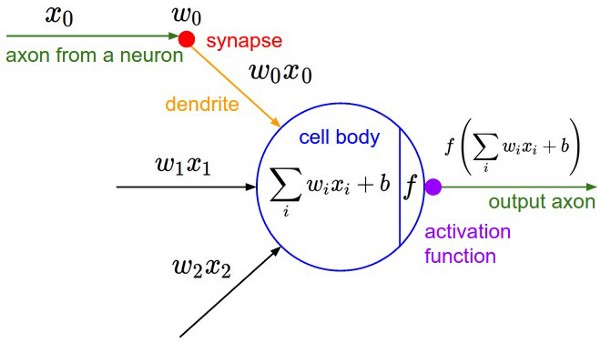
\includegraphics[width=0.5\textwidth]{thesis_template/images/Mathmodel.png}
    \caption{Mathematical representation of a neuron}
    \label{}
    \source{\url{http://cs231n.github.io/convolutional-networks/}}
\end{figure}


 Here the node takes numerical inputs $\mathit{x_0,x_1}$ and  $\mathit{x_2}$ which are assigned with weights $\mathit{w_1,w_2,w_2}$ respectively and calculates the output with the help of a non-linear function \textit{f} which is known as activation function. The main idea behind introducing the activation function is to make the network learn non-linear representations as most of the data in the real world is non-linear. And the Bias \textit{b} decides whether the neuron should fire or not, in simple terms there is no output without it. Bias provides every node with trainable constants.%\cite{IEEE485891}
\subsubsection{\textbf{Now let us see the structure and working of model}}

The network architecture has three different layers which contain set of nodes, they are referred as
\begin{itemize}
    \item \textbf{Input layer:} This is a layer which is essential in introducing different patterns to the network. It just acts as a bridge between data and the hidden layers and there is no modification of data here.
    \item \textbf{Hidden layers:} They are set of layers where all the computations are done. They perform computations by applying different functions and transfer the output in the form of weights to the next layer which can be another hidden layer or output layer. There can be N number of hidden layers whose main job is to transform the data into something an output layer can use.
    \item \textbf{Output Layer:} It consists of a set of nodes that are responsible for collecting the information from hidden layers and then transmits it according to the way it was designed to give to the outside world. And the pattern represented by the output layer can be traced back to the input layer.
\end{itemize}


\begin{figure}
    \centering
    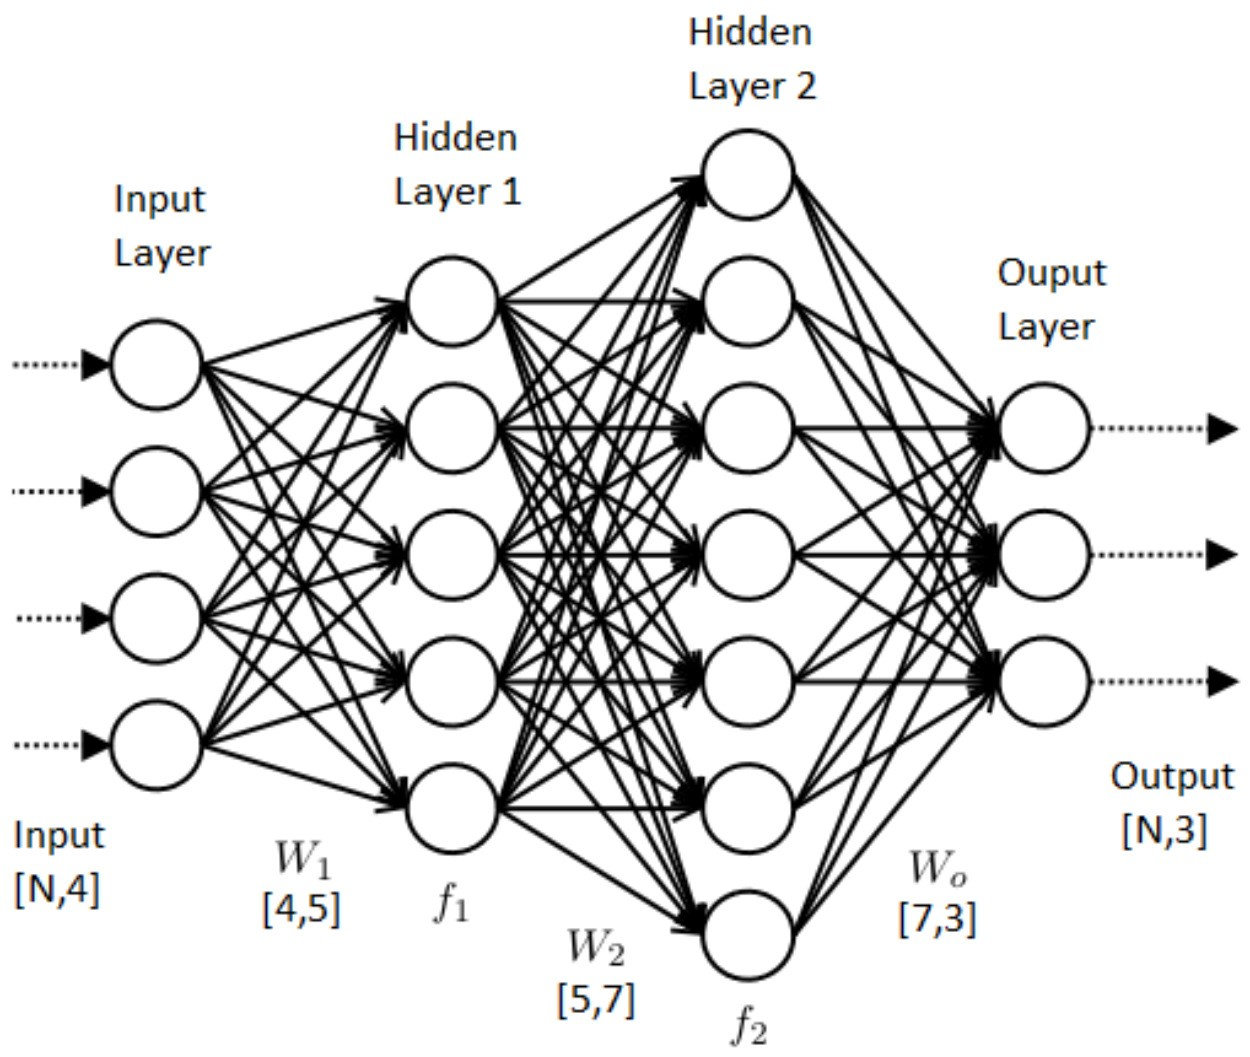
\includegraphics[width=0.5\textwidth]{thesis_template/images/ANN.png}
    \caption{A simple Neural Network}
    \label{}
    \source{\url{https://medium.com/coinmonks/the-artificial-neural-networks-handbook-part-1-f9ceb0e376b4}}
\end{figure}
\noindent The figure represents the basic architecture of a \textit{\textbf{feedforward}} neural network where data enters at the input layers and continues to pass through the network layer by layer where classification is done. There is no feedback between the layers and hence it is called a feedforward network. In an NN output of one layer is the input of another layer.
\subsection{Learning process of Neural Networks}
As mentioned above Neural Networks are about learning from the data and making predictions based on it. Most widely used learning technique is \textit{Supervised Learning} where the input data is already assigned with output labels. The learning process involves different phases as described below
\begin{itemize}
    \item \textbf{Defining Model:} Building the model with random initialization of weights is a very common practice. And later on, through an iterative learning process, the weights can be updated in order to get the ideal model which has the best prediction.
      \item \textbf{Forward pass:} The next step after initializing the model is to check its performance. We start by passing the input we have through the model and calculate the actual output of the model straightforwardly. As the data is flowing in the forward direction it is known as forward pass.
 
     \item \textbf{Calculating the loss function:} By this step, we have actual output calculated by the model but we already have desired output which we want network to learn. In order to achieve it, we first need to calculate Loss, Error or Cost function which is the difference between actual output and desired output.
     $$E(w)= p - p^* $$
     where E is the cost function and \textit{p} is the desired output and $p^* $ is the actual output. Different loss functions calculate different error rates for the same predictions thus it has a considerable amount of effect on the model. Most commonly used loss function is Mean Squared Error which calculates the square of the difference between actual value and the predicted value.
     $$MSE = \frac{1}{2}\sum{(f_i- y_i)^2}$$
     where $f_i$ is the predicted output and $y_i$ is the desired output. The value of this loss function is inversely proportional to the performance of the model.
     \item \textbf{Learning process:} After calculating the error function E(w) we now focus on optimizing the weights in the model which is done by learning algorithm known as \textbf{\textit{Backpropagation}}. It is a first-order iterative optimization algorithm for finding the local/global minima of a cost function. Backpropagation works by calculating the partial derivative of the loss function w.r.t weights at a particular layer $\frac{\partial E(w)}{\partial w}$ applying chain rule in calculus.%\cite{IEEE118638}
    \begin{figure}
    \centering
    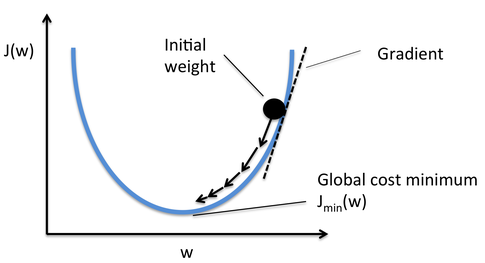
\includegraphics[width=0.6\textwidth]{thesis_template/images/backprop.png}
    \caption{Backpropagation curve}
    \label{}
    \source{\url{https://medium.com/datathings/neural-networks-and-backpropagation-explained-in-a-simple-way-f540a3611f5e}}
    \end{figure}
     
    
    \noindent Basically backpropagation focuses only on calculating the gradients and gives you the direction in which you minimize the error. But updating these weights can be handled using different optimization techniques like gradient descent,stochastic gradient descent or Adam optimizer. The updated weight is
    $$w_1 = w_0 -  \alpha . \frac{\partial E(w)}{\partial w} $$
    
\newpage\noindent In the above formula $w_1$ is updated weight, $w_0 $ is an old weight, $\frac{\partial E(w)}{\partial w}$ is gradient of loss function w.r.t $w_0 $ and $\alpha $ is learning rate a hyperparameter which is randomly given by the user to control the adjusting of weights. The learning rate should not be too low nor too high in order to make sure that we are not missing the local minima.
     \end{itemize}
     This is the common learning process of a Neural Network\cite{IEEE118638}. Now coming to the special kind of Neural network called Convolutional Neural Network which is the type of ANN used in this thesis.
    \subsection{An Intuitive Introduction to Convolutional Neural Networks}
    A specific kind of deep neural networks is Convolutional Neural Network commonly referred to as CNN or Convnet. Inspired by the research of D.H.Hubel and T.N.Wiesel in the 1950s and 1960s which suggested a new model for how mammals visually perceive the world Convolutional Neural Networks are developed. These models belong to a class of ANNs that are designed specially to analyze visual imagery. %\cite{lecun}
    
    Generally, it is very complex to flatten the image and feed it to the normal Neural Network as it requires a large amount of parameters to define this kind of network. Therefore CNNs are proposed to solve tasks related to visual analysis. Unlike regular ANNs where each and every neuron of one layer is connected to other layer, CNNs have a different structure. Firstly the layers are arranged in \textbf{3 dimensions:width,height and depth}. Next, the neurons in one layer do not connect to all the neurons in the next layer but only a small region of it is connected because it will be computationally very expensive if all the neurons are connected. Lastly, the final output will be reduced to a single vector of probability scores which is organized along the depth dimension. This probability score decides the class of an image%\cite{OSheaN15}. The structure is shown in \textit{figure 1.4}
    
     
      \subsubsection{Convnets have two parts}
     \begin{itemize}
      \item \textit{\textbf{Feature extraction}}, which is performed in hidden layers where different patterns/features are learned from the given input image.
      \item \textit{\textbf{Classification}}, involves few fully connected layers which serve as a classifier for the extracted features. They assign a probability for the object on the image.
         
     \end{itemize}
     \subsubsection{\textbf{Architecture of CNN:}}
   
      \begin{figure}[h]
    \centering
    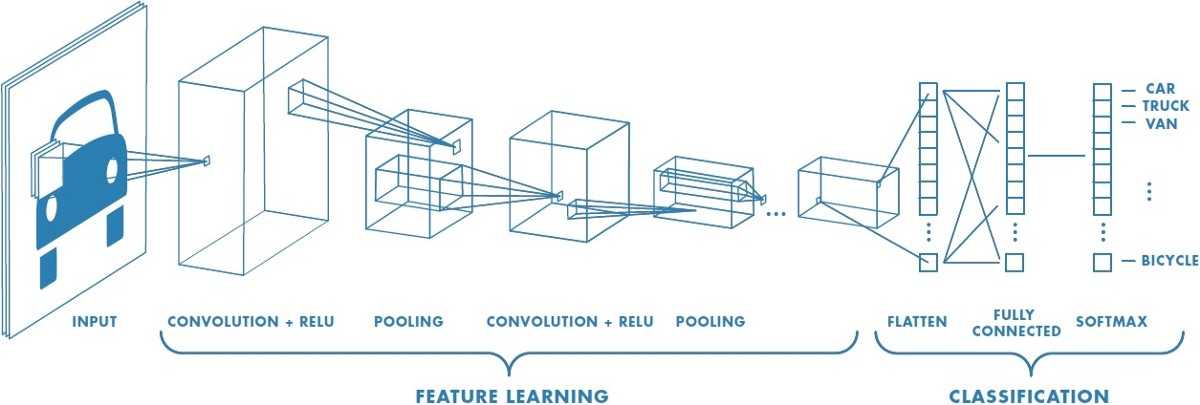
\includegraphics[width=1\textwidth]{thesis_template/images/CNN.jpeg}
    \caption{Structure of a CNN }
    \label{}
    \source{\url{https://www.mathworks.com/videos/introduction-to-
    deep-learning-what-are-convolutional-neural-networks--1489512765771.html}}
    \end{figure}
 \newpage  \subsubsection{\textbf{Working of the network:}}
     When we feed the network with input image the following operations are performed sequentially by the network:
\begin{itemize}
    \item \textbf{Convolution Layer:} Convolution generally means merging of two things to produce a different thing. Most of the heavy computations are done at this layer. The layer consists of a set of learnable \textit{filters or kernels or weights} each learning to look for something different in an image. And during the forward pass, each filter is slid across the width and height of the input to produce an activation map. Numerous convolutions are performed here as each filter is convolved only with a small region of input and this results in many activation maps. All these maps are put together as a final output of the layer.%\cite{8308186}
    
   The layer also consists of two hyperparameters that control the output volume or their spatial arrangement. Firstly we must specify \textit{\textbf{Stride}}, it is the size of the step the convolution filter moves each time. For example, if the stride value is 1 it means that the filter moves pixel by pixel. The larger stride results in the smaller output volumes spatially.\cite{8308186}
   
 \setlength{\parindent}{10ex} Secondly,\textit{\textbf{Zero-padding}} which means the addition of zero value pixels surrounding the input image. Because the feature map is always smaller than the input this is done in order to prevent it from shrinking. Doing so also helps in increasing the performance of the model.\cite{8308186}
 \item \textbf{Activation layer:} Activation functions help Artificial Neural Network to learn and make sense of something really complicated and Non-linear complex functional mappings between the inputs and output variable. This layer determines the output of the filter i.e., whether it should fire or not. The activation function is always non-linear in order to make it easy for the model to generalize or adapt to a wide variety of data. The non-linear function graph is represented as below.
 \begin{figure}[h]
    \centering
    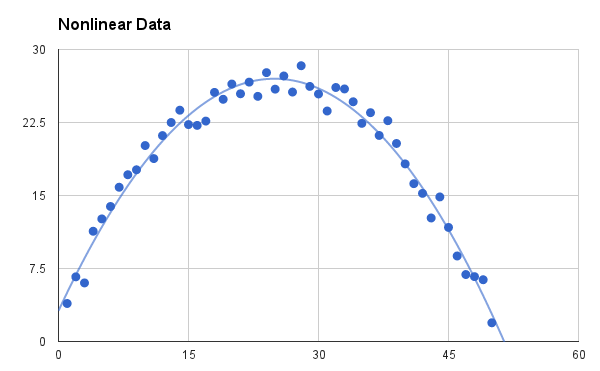
\includegraphics[width=0.5\textwidth]{thesis_template/images/nonlinear.png}
    \caption{Non-linear graph}
    \label{}
    \source{\url{https://towardsdatascience.com/activation-functions-neural-networks-1cbd9f8d91d6}}
    \end{figure}
 
 
 \newpage\noindent There are so many activation functions like \textit{\textbf{Sigmoid}}, \textit{\textbf{Tanh}} but  \textbf{\textit{ReLU}} is the most commonly used activation function  by CNN just like any other Neural Network to produce non-linear output. This layer maps the function $f(x) = max(0,x) $. This function changes all the negative outputs to zero. It is very important as negative values also contribute to the output of the next layers which means the absence of the feature. But it does not have any effect on the shape of the image.\cite{8308186} 
 \item\textbf{Pooling Layer:} Image processing is a very computationally intensive process. In order to allow our model to run at a decent speed while not compromising on accuracy too heavily, we do a form of dimension reduction on the image size in a technique called pooling. It is very important to have a pooling layer between two successive convolutional layers whose function is to reduce the spatial size of the representation.\\
 \begin{figure}[h]
    \centering
    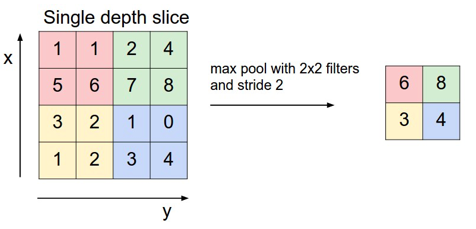
\includegraphics[width=0.5\textwidth]{thesis_template/images/maxpool.png}
    \caption{\small Max-pooling}
    \label{}
    \source{\url{http://cs231n.github.io/convolutional-networks}}
    \end{figure}\\
 The most commonly used pooling is \textbf{\textit{max-pooling}} which considers the maximum value in each window without losing the significant information. This layer reduces the amount of parameters and computations in the network. The most common form of a pooling layer has filters with a size of $2*2 $ with a stride of 2 which discards atleast 70 percent of activations. This layer also works alot like convolutional layer.

  
    
    \item \textbf{Fully-connected Layer:} After the convolution and pooling layers the important task of classification is done by fully-connected layer. The main goal of these layers is to flatten the features that are learned by the convolutional layers. All the neurons in these layers are connected to all the activations in the previous layer and they convert 3D data to 1D data into a set of probabilities. The most commonly used function for the conversion of the data is \textit{softmax function}, it gives the set of discrete probabilities for each class we are trying to predict. It computes the probabilities of each target class over all possible classes. It can be mathematically expressed as follows. 
    $$\sigma(y_i) = \frac{e^{y_i}}{\sum_{j=1}^{N} e^{y_j}}$$
     Where N is the number of classes. Next we use $argmax(\sigma (y_i))$ function to map the input image $x_i$ to its class $y$.\cite{8308186}
    \end{itemize}
    All these steps contribute to one forward pass of an image in the network. The training of a CNN is done using backpropagation gradient descent algorithm.
  
  
  \section{Problem Statement:}
   Ever since their introduction during the early 1990s by Yann LeCun\cite{lecun} Convolutional Neural Networks have been performing very well in tasks related to computer vision and almost reached human-level performance. Especially because of their parameter sharing they can be used in any device. The incredible speed of research in this area combined with the open availability of GPUs and large databases has given impressive results in past few years. Now CNNs are one of the important non-linear models that are used in most devices starting from face recognition in your phone to Google self-driving cars\cite{Al-Qizwini} and they are the go-to model for every image related problem. In terms of performance, they have achieved superhuman accuracy which means that they perform better than humans. 
   
\noindent   Now, the problem with these models is though their performance is very impressive sometimes it is difficult to understand what and how exactly these large models are learning. For this reason, they are often considered as black-box models. And without understanding the internal working of the network it is hard to trust them. For example, let us assume that we are training the network with images of bedroom, now the question is what is the model specifically looking for. It may classify the image just by looking for a bed or lamp or a table, so now next time whenever it detects a table there is a possibility that it classifies the image as bedroom. But it might be an office image, now the model has done wrong classification. The technique to overcome this type of problems is visualization of trained filters. Visualizing the nodes inside the network solved many problems related to these deep models. Lately, there is a lot of research going on in this field of visualizing what is happening inside the network.
  \subsection{Need to Visualize}
   \begin{itemize}
       \item To understand how the model is making these predictions.
       \item To see if parameters and hyperparameters are chosen correctly and if not tune them for obtaining better models.
       \item Ensure if all the filters are learning because in some cases filters might converge to zero which means that they are not really being used.
       \item Also helps in debugging the model.
       \item To tell where the network has been saturated. 
   \end{itemize}
\newpage   \subsection{Research Questions}
   This thesis includes answering the two questions mentioned below:
\begin{itemize}
    \item \textbf{Visualize the hidden layers of the Convolutional Neural Network:}
    
    This includes visualizing the weights of the trained model and also look if different parameters and the hyperparameters have any effect on the learning patterns of the nodes. The main part of this thesis includes only convolutional layers so fully-connected layers are ignored. 
    \item \textbf{Looking for the redundancy in the network:}
    
  We say the network is redundant when two or more filters or layers in the network learn the same pattern. And a redundant network consumes a lot of computation time and effort. The work also includes finding out if there are redundant filters in the network and if so what kind of parameters are causing it. 
\end{itemize}


    

    
     
     
     

     
     
     
     
     
     
     
 







\chapter{Background}\label{chap:background}
\section{State of the Art CNN Architectures}
During the past 2 decades many number of CNN architectures were designed. The first CNN architecture known as LeNet-5 was introduced in the year of 1998 by Lecun. This architecture has seven layers with 60k parameters and its main goal was to recognize hand written digits.However the network was constrained because of its inability to perform well on high resolution images.

The need for a CNN model that can also compute high resolution images lead to the development of more sophisticated architecture known as AlexNet. This was the time when neural networks gained their prominence.  The availability of GPUs and large data sets made it faster and easier to develop these kind of models. This architecture was introduced in the paper\cite{Krizhevsky} in the year 2010 which outperformed all the previous architectures. It is similar to LeNet-5 except it is more deeper with 60M parameters and with stacked convolutional layers. It has $224\times224\times3$ input layer with $11\times11 $ filter size with a stride value of 4. It was trained on Imagenet dataset which has over 15M high resolution images along with their labels.Their network topology was a bit complex because of bigger receptive fields and stride value.  According to \cite{Krizhevsky} this model achieved error rate of 17.0\%. Later on they entered a competition ILSVRC 2012 a large scale image recognition challenge and achieved a winning top error of 15.3\%. 

The next architecture was introduced by Visual Geometry Group and it is VGG16 with 16 layers. The work by \cite{SimonyanZ14a} proposed this architecture and concluded that the depth of the Convolutional Neural Network has an effect on its classification accuracy. Unlike \cite{Krizhevsky} this architecture has a very less receptive field of $3\times3$ and hence focuses on each and every part of the image. This architecture has won best classification in ILSVRC 2014. There is also VGG19 network which has 19 layers.

\noindent However as the state of the art networks keep getting deeper and deeper a new problem was discovered. Which states that when we are training a deeper architecture as the gradient is propagated to earlier layers repeated multiplication may make gradient to appear smaller or vanish totally and also accuracy gets saturated and then starts to degrade. Motivated by the thought of attacking this problem another type of network called ResNet(Residual Networks) was introduced by Kaiming He \cite{ResNet15}.This model achieved top error rate of 3.57\% and was the winner of ILSVRC 2015. Though this network is much deeper than the previous networks its complexity is lesser because they introduced a new idea of "Skip connections" it means that instead of trying to learn the direct mapping of $x$ to $H(x)$ we can calculate the residual say $F(x)=H(x)-x$ between two and then make the network to learn $F(x)+x$\cite{ResNet15}. These networks also solve vanishing gradient problem by making the gradient backpropagate through shortcuts.

ResNets totally changed the way we understand a Neural Network. This architecture paved the way to develop CNNs with hundreds of layers. These are the different type of CNN architectures that has achieve state of the art results in the field of computer vision.
\subsubsection{\textbf{\textit{Complications with the architectures}}}

Undoubtedly CNNs have almost reached the human level performance in the tasks like image recognition,classification etc.,despite of their impressive work there are still so many things that are unclear like what are the factors that contribute to the precise computations and the internal workings of the network.  Provoked by these problems lately lots of research has been done to propose different techniques that helps us visualize the internal structure of the network. Erhan et al\cite{Erhan09} made few contributions to the idea of visualizing the internal computations of the network to gain some intuitions about it. The work focused on \textbf{activation maximization}, a technique used to find the part of input image that is responsible for the units maximum activation. Usually while training a network the weights are updated iteratively but input and output image remains constant but in this technique the weights and output image are kept constant but input image is modified such that it maximizes activation maps of certain neurons. However this method was not effective in determining networks invariance.  


Next the work of Zeiler et al \cite{zeiler11} which was about reconstructing the input from the output using top down approach and in an unsupervised manner. They used the concept of deconvolution and reconstructed images at each layer with the help of filters and switch variables. These switches are located between the feature maps and pooling layers and thus they can be used during unpooling and restore the original image.  In their method they visualize each kernel by considering respective activation map and pick the image that causes the maximum activation and project it down to input space. 


Based on this work Zeiler \& Fergus et al\cite{zeiler13} developed an improvised version of deconvolution for visualizing the layers inside the network. Previously Deconvnets was used only for unsupervised data in this work they developed the \textit{Deconvnet} model for supervised data. They used multi-layered deconvolution network to project the feature maps back to the input space. Their approach had Unpooling of layers with the help of switch variables to produce feature maps and then these maps are rectified using Relu activation and then convolved with the transpose of the filters. This concept is similar to \textit{encoder-decoder}. In their method they used a pre-trained network Alexnet\cite{Krizhevsky} whose kernels were trained on \textit{ImageNet} dataset which has 1.3 million images over 1000 different classes, instead of training the network from scratch. While visualizing the architecture they were able to discover problems with the model and they changed the architecture of the first layer by reducing the filter size from $11\times 11$ to $7\times7 $ and stride to 2 in both first and second layers. Occlusion sensitivity analysis was also conducted by covering different parts of image with gray scale in order to find out which portions of the image are contributing for the classification. During visualization of internal structure of the model they also found that there exists some degree of correspondence in the network. They have conducted ablation study by removing fully connected layers and different convolutional layers and concluded that depth of the model plays a crucial role in the performance of the model. 

Next in the year of 2014 \textit{Zhou et al}\cite{Zhou14} have revolutionized the method of occluding the images \cite{zeiler13}. In this work instead of using a single gray patch for occluding the images they replicated each image by occluding many regions of it by randomized pixel values. This approach allows to analyze the important regions of an input image that are responsible for the activations produced by each unit. It also suggests that the units in the hidden layers act as object detectors of an image though there is no specification provided on the particular region of the image.

Next comes \textit{Zhou et al}\cite{Zhou15} proposed a new technique known as Class Activation Map(CAM) where an activation map is reconstructed in the previous layer by mapping the predicted class score back. This technique helps in highlighting the class specific regions which means finding the particular region in the input space that contributes more for the classification. Here the authors evaluated their work on CNNs that perform global average pooling on the convolutional feature maps just before the classification/output layer. However their work contributed more towards object localization of an image.

The other way to look in to the hidden layers of CNN was put forward by \textit{Simonyan et al}\cite{Simonyan13}. Here the authors backpropagated the class score back to input space and they proved that doing so helps in finding the pixels that are contributing most to the classification. In this way we can know if the non-linear model is looking at the main object or other parts of the image.

In \cite{Felix} the above described techniques for visualization of Convnets are classified in to three types \textit{Input Modification, Input Reconstruction } and \textit{Deconvolution}. In this work the authors developed a library called FeatureVis built on top of MatConvnet toolbox to implement and also compare the above described techniques. This library is also used in comparing different bigger architectures like GoogleNet, Vgg16 etc. All the previous have already taken the existing architectures and then visualized the internal structure of the network.

Motivated by the previous works this thesis includes visualization of the filters after training the network. It involves building and training the non-linear network from scratch instead of considering pre-existing models. This thesis is more about finding out the effect of different parameters and hyper parameters on the feature extraction part of the network. And only focused on convolution layers so densely connected layers are ignored.
\chapter{Methods}\label{chap:methods}
\section{Workflow of Visualization of Network}
Below is the sequence of steps that I followed during the implementation. For this I have used python with Keras. 
\begin{figure}[h]
    \centering
    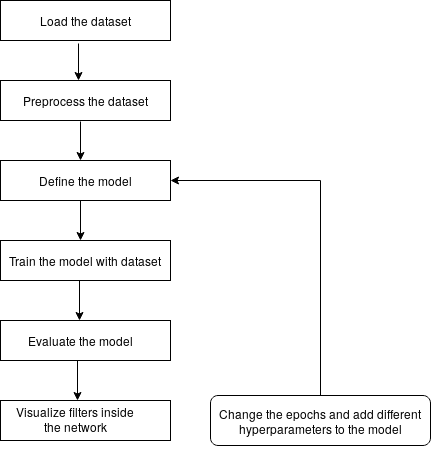
\includegraphics[width=0.7\textwidth]{thesis_template/images/flo.png}
    \caption{\small Flowchart representing steps followed}
    \label{}
    \end{figure}


\newpage \noindent \textbf{Reason to choose Keras}\\
 Keras\footnote{\url{https://keras.io/}} is an API which is built on top many other frameworks like Tensorflow, Theano and CNTK. This framework makes it easy to build bigger deep learning models with many layers with less time. It also has many pre-defined parameters and hyper parameters so we need not define each and everything in detail. 

And most importantly the main part of this work is to visualize the filters inside the model and Keras-vis\footnote{\Url{https://raghakot.github.io/keras-vis/vis.visualization/}} is used for this, so keras was used to build the models. As keras is built on the top of tensorflow later on we can also convert it into tensorflow model if needed. Finally my experience was I was able to apply many different optimizers and activation functions without any difficulty. And I got time to build and experiment on many different models.\\
PS: I have not described all the models in this section.

\subsection{Loading the dataset}
 
The dataset is MNIST which was introduced by Yann LeCun, Corinna Cortes and Christopher Burges \cite{LeCun}. It is a dataset that contains hand written digits which is a subset of larger dataset from NIST. The dataset must always be divided in to train and test dataset in order to train the model on training images and then evaluate its ability of image classification on test set. MNIST already has 60000 train images and 10000 test images which are of size $28\times28$ and are gray scale images i.e.,only one channel. Which means the height and width of an image is 28 and depth is 1. 
 
\noindent In keras it is very easy to download the dataset as it comes with a library of datasets. It has data which is already split in to train and test data and once we load the dataset X\_train, y\_train, X\_test, y\_test are loaded where X indicates images of train and test data and y indicates respective labels.

In order to go to the next step we need to have a clear understanding of the dataset. Using plot method we can look at the images to check if the data is correct. 
\begin{figure}[h]
    \centering
    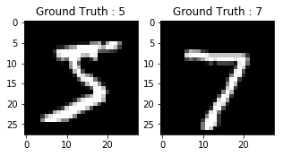
\includegraphics[width=0.5\textwidth]{thesis_template/images/screenshot.png}
    \caption{\small Random images from the dataset}
    \label{}
    \end{figure}
    
 
\newpage \section{Preprocessing the data}

This is the main step in training the model with the data because we need to convert the data in such a way that model can extract features from it. 
\subsection{Reshaping the data}
From above image it is clear that the images are in grayscale that have pixel values in the range of 0 to 255.
The data have $ 28\times28 $ dimensions hence it should be reshaped in to the form of (28,28,1) in order to feed it to the network. 

Here Tensorflow is the backend therefore the channels come last. In case of Theano the channels come first. We need to be very careful in the image dimension ordering before feeding the data to the model otherwise the model cannot take the data.


\noindent As Convolution2D layer in Keras accepts an input of 4D tensor with shape (batch, height, width, channels) if data format is "channels\_last". In this case this is done by  X\_train.reshape(-1,28,28,1), here -1 indicates that the batch size can vary. 

\subsection{Rescaling the pixel values}

In order to reduce the computational complexity we need to rescale the pixel values of the images in dataset. The pixel values range from 0 to 255 where 0 is black and 255 is white. Since 255 is the maximum value we need to divide the images by 255 so that the resulting pixels are in the range [0,1]. 
\newpage\noindent We do this in order to normalize the image values because some images have high pixel values and some have very low pixel values. Normalizing the input values to the same range lets all the images contribute evenly to the total loss as all the images in the dataset are sharing the same model and same weights. Without scaling it will be hard for the model during training to update the weights.

Scaling the pictures in same range of [0,1] helps us using only one learning rate, otherwise higher pixel values need smaller learning rates and lower pixel values need larger learning rates. Since the dataset I used has small dimensions of $28\times28$ rescaling is done by dividing it with 255, for images with higher resolution the values might vary. There is also one more thing we need to consider here the data we have is in uint8 format, now we have to convert it to "float32" format.

\subsection{One-hot encoding of labels}

Convnet model cannot operate directly on the labels of the images so we use one-hot coding to convert this categorical data in to a numerical form. It means we are creating dummy variables from categorical data. Here one-hot encoding will be a row vector of $ 1\times10 $ dimension.

 It means that the vector consists of all zeroes except for the class it represents. For example an image of class 1 has a label of [1 0 0 0 0 0 0 0 0 0].
\subsection{Splitting the training set} 
Now we have training data and testing data which is preprocessed in such a way that CNN can accept and learn from it. But there is one more vital step that is to split the training data properly in to training and validation data. Basically this is done to reduce overfitting and increase the generalization ability of the model. It can be split in to 80\% training data and 20\% validation data so that we can validate the model on the data which it has never seen before, doing this also helps in efficient performance on test data. Let us now take a look at how our data looks.


Here we have 48000 training images and 12000 validation images of shape (28,28,1)
\section{Defining the model}
This involves defining a basic model with just Convolution,relu and pooling layers. No extra regularization techniques were used here.
This step involves creating a model. Building a machine learning properly plays an important role in image classification. The structure of the model determines the performance of it. The beauty of this Convnet is we can model it according to our wish i.e., we can put as many hidden layers as we wish. In order to answer the problem statement just need few hidden layers are needed so the model is not so deep.
The model is Sequential stack of layers. I have used four Convolutional layers.
\begin{itemize}
    \item \textit{\textbf{First Convolutional layer}} will have 16 number of filters with the size of $3\times3$ which takes the input of size (28,28,1)
    \item \textit{\textbf{Second Convolutional layer}} will have 32 number of filters of same size as first layer.
    \item \textit{\textbf{Third Convolutional layer}} will have 64 number of filters of same size as previous layers.
    \item \textit{\textbf{Fourth Convolutional layer}} will have 128 number of filters of size $3\times3$ 
    \end{itemize}
\textbf{\textit{Why increasing number of filters? }}\\
The pattern of selecting the number of filters in each convolutional layer is similar to vgg16 model which has even and increasing number of filters. The layers have increasing number of filters as we go deep in to the network in order to increase the representational power of the network. Second reason is in convnets we downsample the images as we go through the network to tolerate this resolutional loss we increase the number of units. 
 \textbf{\textit{What does every convolutional layer consist of? }}\\
 Every Convolutional layer two very important hyper parameters i.e., padding and stride values. The importance of these two is explained in the Introduction. Keras can understand zero padding as "\textit{padding = same}" and with a stride of 1. \\
  PS: The most important thing observed here is when padding was not included in the convolutional layer the input got shrunk within three layers and it went in to negative values. This resulted in very shallow model and in turn the accuracy was effected. So padding is a very important hyper parameter especially when images are of low resolution. \\
  In addition to these convolutional layers there are also Relu and Max-pooling layers after each Convolution layer. Sequentially it has convolution layer followed by Relu layer followed by Max-pooling layer of size $2\times 2$.\\
  $$Conv2D\rightarrow Relu \rightarrow Maxpooling$$
  
\subsubsection{\textbf{\textit{Why only ReLU activation layer? }}}

Relu is selected over other activation functions because it is always either positive or zero but not negative. Both the activation function and its derivative is monotonic. This makes the computation cheap and helps the network converge faster without effecting the accuracy.
 \begin{figure}[h]
    \centering
    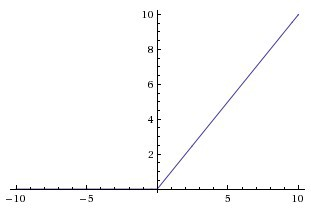
\includegraphics[width=0.5\textwidth]{thesis_template/images/rElu.jpg}
    \caption{\small Relu graph}
    \label{}
    \source{\url{https://medium.com/the-theory-of-everything/understanding-activation-functions-in-neural-networks}}
    \end{figure} 

\noindent The range of ReLU activation is [0,$\infty$). The graph of ReLu looks like linear but it is generally non-linear in nature.  And one more reason to use this function is to overcome the problem of \textit{Vanishing Gradient} which occurs especially when we use gradient based optimization methods.
\\ \textbf{ \textit{Vanishing Gradient problem:}} Convnets basically suffer from the problem of decreasing gradients when we are using more complex data like images. Now during the training process of a large networks using back-propagation the model calculates gradients of loss with respect to each trainable parameter and as we move backward the magnitude of gradients gets exponentially smaller and can also vanish completely. This happens when the activation function squashes the input in to a very small output range (0,1) and you further multiply it by even smaller learning rate. This in turn effects the value of delta to be updated and lower layers will get little or no updates. If there is a small update then the network would require larger training time and when there is no update the network cannot converge at all. The diminishing of this gradient values is referred to as vanishing gradient problem. When we use activations like sigmoid or tanh this occurs. According to \cite{Ide} the smarter and easier way to overcome this problem is by using the Relu activation as it is always positive and maps only the maximum value.\\ 

\noindent After the four convolutional, relu and pooling layers the model had two fully-connected layer followed by softmax layer.

\subsection{Compiling the model}
The model is ready now, next we have to train it using the preprocessed data. For that first we need to compile the model using the loss function and the optimizer. To compile the model we need to consider three parameters i.e., loss function, optimizer and metrics. \\
 \textbf{Loss Function:}
Here "Cross entropy" is the loss function I have used instead of Mean square error since it is already defined in Keras we can just import it. The binary cross entropy is defined by the following formula\\$$H(p,q) = -\sum_{x}p(x)log q(x) $$ \\
Here probabilities are represented by 'q' and labels are in 'p' slot. In case of CNNs and for problems like classification this loss function is more used because the output of the model is probability distribution (output layer in the model is softmax which is a set of probabilities). The lower value of this loss function indicates that the model is performing better.\\
\textbf{Optimizer:}The optimizer controls the learning rate of the parameters. The learning rate determines how fast the optimal weights for the model are calculated. Adaptive Moment Estimation(Adam) \cite{Diederik} optimization method is used here which is an extension of RMSProp optimization algorithm with momentum. \\
\noindent\textbf{\textit{Adam}} uses two tricks which makes the network to converge faster. \cite{Diederik} They are \begin{itemize}
    \item Momentum: It means that some fraction of previous update is added to current update in a way that repeated updates in one direction compound. There is no need to add momentum as a hyper parameter like in SGD as adam already incorporates it.
    \item Adaptive learning rate: It means that it uses learning rate according to the parameter. This is beneficial because the parameters in the early layers need higher learning rates and it makes sense to increase learning rates only for those parameters. This speeds up the learning. And the learning rate does not need manual tuning in this algorithm. 
\end{itemize}
For every weight $w^j$ adam calculates
$$ v_t = \beta_1 * v_{t-1} - (1- \beta_1)* g_t $$
$$ s_t = \beta_2 * s_{t-1} - (1- \beta_2) * g_t^2 $$
$$ \Delta w_t = -\eta \frac{v_t}{\sqrt{s_t + \epsilon}} * g_t $$
$$ w_{t+1} = w_t + \Delta w_t $$
Here $\eta $ is learning rate, $g_t$ gradient at time t, $v_t$ and $g_t$ are exponential averages of gradient and gradient squares respectively. The parameters $\beta_1 $ and $\beta_2$ are exponential decay rates of first and second moments respectively. We used standard values of these two parameters as proposed by the authors i.e., 0.9 for $\beta_1$ and 0.999 for $\beta_2$. And the other parameter is learning rate or the size of step which has very small value. \cite{Diederik} \\
\noindent\textit{\textbf{Why is Adam better than SGD?}} \\
SGD maintains a single learning rate throughout the training process but Adam computes  individual adaptive learning rates for each parameter from estimates of both first and second moments of the gradients. It means it does not adapt learning rates just based on first momentum but also considers the average of second momentum. Adam learns the learning rate itself on per-parameter basis. 



\section{Training the model}
Now we have both data and the model now its time to train the network. To train the network here we use 'fit()' function on our model with different parameters like training data X\_data and validation data along with batch size and number of epochs it should be trained. 


\noindent In order to visualize the performance of the model during the training process after each epoch we define history. The batch-size and the number of epochs can be changed and they have huge effect on the accuracy and performance of the model. It means that more number of times we pass the data through the network more accurate it will perform. 
While doing this we can see the training and validation accuracy and loss of the model. Next we can test this machine learning model by using it to make predictions on test data(model.predict() method is used for this).\\ 
  But accuracy alone is not enough to evaluate the model. Because it hides the details we need to better understand the performance of our model. Especially when we are dealing with multi-class classification we need to know if the images are predicted correctly or not, for this we need to validate our model's performance using precision, recall and F1 scores. The detailed explanation for these metrics is described in the next section.


\section{Evaluation of model using different metrics}
\subsection{Confusion-Matrix}
\textit{What is confusion matrix?}\\
As the name suggests it is a matrix that tells how many times your model was confused while making predictions. It gives the deeper intuition on the performance of any machine learning model. The matrix helps you determine what are the categories that you often get right and much more importantly, which are the ones you often get wrong. To understand confusion-matrix and other metrics which are described in further sections we need to understand these terms \textit{true positives,true negatives, false positives and false negatives.} \cite{inproceedings}
\begin{itemize}
    \item \textbf{True Positive(TP):} The model predicted positive and it is true.
    \item \textbf{True Negative(TN):} The model predicted negative and it is true.
    \item \textbf{False positive(FP):} The model predicted negative but it is true.
    \item \textbf{False Negative(FN):} The model predicted negative and it is false.
    \end{itemize}

The matrix consists of these values. For example a basic binary classifier has a confusion-matrix that has these values as follows.
\begin{figure}[h]
    \centering
    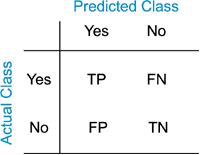
\includegraphics[width=0.4\textwidth]{thesis_template/images/con1.png}
    \caption{\small Confusion-matrix}
    \label{}
    \source{\url{https://en.wikipedia.org/wiki}}
    \end{figure}\\
The matrix has
\begin{itemize}
    \item Rows: Which represent the actual class.
    \item Columns: Which correspond to the predicted class.
\end{itemize}
\noindent In a multi-class classification model confusion-matrix gives a clear visualization of how many images in the dataset are predicted correctly. To calculate this we need a validation dataset with expected outputs. 
 The number of correct and incorrect classifications are filled in the table. The total count of correct predictions for a class go in to the expected row and predicted column for that respective class. In this case the model is trained on 10 different class and achieved accuracy of 99.8\% on test dataset. To calculate confusion-matrix Skicit learn library is used. 


 \subsection{Precision, Recall and F1-score}
 
\textit{\textbf{Precision}} also called Positive Predictive value is the ratio of number of True Positives predicted by the model to number of True Positives and false positives. 
$$ Precision = \frac{TP}{TP+FP}$$
This score tells us how precise our model had made classifications and for every class how much it predicted correctly. It should be as high as possible. \\

\noindent \textit{\textbf{Recall}} also called as Sensitivity or True Positive Rate is the number of True Positives divided by the number of True Positives and number of False Negatives. 
$$ Recall = \frac{TP}{TP+FN}$$
So it can be understood as a measure of classifiers completeness. The value should be as high as possible otherwise it indicates many False Negatives.

\noindent \textit{\textbf{F1-Score}} is the harmonic mean of Precision and Recall. It takes both False Positives and False Negatives in to account. It uses harmonic mean instead of arithmetic mean by punishing extreme values more. It is difficult to compare two models with low Precision and high recall or vice versa. So to make them comparable we use F1-score. It measures both metrics at the same time.
$$F1 = 2* \frac{Precision*Recall}{Precision+Recall} $$

\noindent F1-score is more useful than accuracy of the model as it considers both False Positives and False Negatives. \cite{scikit-learn}







\subsection{AUC-ROC Curve}
Another most popular metric is ROC which is Receiver Operating Characteristic curve which helps us in visualizing the performance of a machine learning model. An ROC curve plots true positive rate(TPR) on the y-axis versus false positive rate(FPR) on the x-axis. It shows how the TPR and FPR values vary as we modify the threshold for identifying a positive in our model. The value of threshold is changeable.

\noindent Here TPR is Recall. To understand FPR we need to know Specificity which is 
$$ Specificity = \frac{TN}{TN+FP} $$
$$ FPR = 1 - Specificity$$

\noindent AUC means Area Under Curve which represents the measure of seperability. It gives us an intuition about how much the model is able to distinguish between diferrent classes. By calculating AUC we can quantify the model's ROC curve \cite{Yang}. All these performance metrics obtained for this model are shown in the results section.
 


\section{Visualizing the filters inside the network}
The first important thing is the method involves visualizing convolutional layers, fully-connected layers are not included. Keras makes it easy to save and load the model, this avoids training it multiple times and saving time.

 \subsection{Visualizing by Activation Maximization} The first method is finding the input image that maximizes the activation of a filter. It is an activation based method. The idea is that every filter is capable of learning different patterns from the input image and we need to generate an image that produces high output activation for that filter. Keras-vis library is used for this which has $visualize\_activation$ API to visualize activations of the filter. The method is known as activation maximization \footnote{\url{https://raghakot.github.io/keras-vis/visualizations/activation_maximization/}} and it calculates $$ \frac{\partial ActivationMaximization Loss}{\partial input}$$ 
Before proceeding further keras-vis should be installed. Now we need to know the layer names of each layer to make it easy for us to know which layer we want to visualize and model.summary() provides this facility. It gives us the clear picture of name and number of parameters in that layer. For this use case we need to use visualize\_activation to look at what filters are recognizing. 

 \noindent The most important thing to understand about this method is that filters and output are kept constant and input is modified so that it maximizes certain units in the model. First activation layer was chosen to visualize which has name 'activation\_1'. For this method layer\_idx and filter\_indices are the important arguments where layer\_idx indicates the index of layer that need to be visualized and filter\_indices refer to the index of filter in the  layer. Here layer\_idx is set to convolution layer. 

\begin{figure}[h]
    \centering
    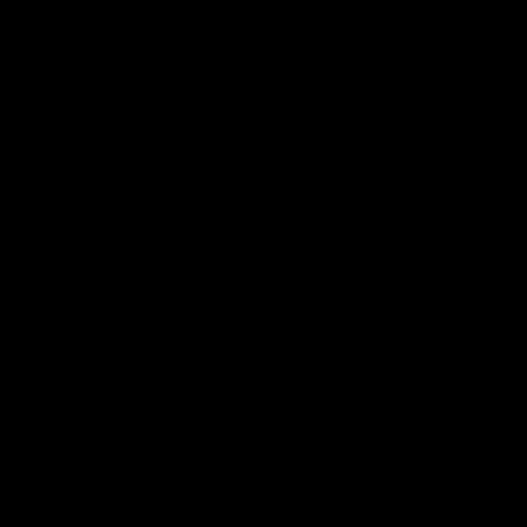
\includegraphics[width=0.6\textwidth]{thesis_template/images/stitchedfilter.png}
    \caption{\small stitched filters of first activation layer}
    \label{}
    \end{figure}

\noindent By using this method on first activation layer it gave the output which was totally black. The image below represents the outcome of this method. For different layer\_idx and different images it gave the same outcome. 

\newpage \noindent This is the reason why next method was taken in to consideration. It is visualizing the filters of individual layers. This is possible by defining a method for plotting the filters. 

 \subsection{Visualization of Intermediate layers}

Here comes the interesting part of this work, to achieve first layer visualizations we have to define a function which takes one argument which is layer name\footnote{\url{http://cs231n.github.io/understanding-cnn/}}. This method made it easy to visualize the filters inside each layer given particular image. For this random images can be chosen from the test dataset and then visualize the features of that image in the network.
 To understand more clearly this model has 32 filters in the first layer. Hence for the image generated randomly there were 32 different activations where each activated filter was again an image. 
 
 
 The outcome of this experiment is discussed in the results section. In addition to this the section consists of the visualizations of slightly modified model with different parameters.  



    
\chapter{Results}\label{chap:results}
 \section{Different performance metrics of Model}
The network is very simple with following parameters.
 \begin{itemize}
     \item \textit{Activation:} Relu
     \item \textit{Optimizer:} Adam
     \item \textit{Filter size:} $3 \times 3 $
     \item  25 epochs and 200 batch-size
     \item \textit{Dataset:} MNIST
\end{itemize}
 Now let us look at the variation of accuracy and loss during the training.
 
\begin{figure}[h]
    \centering
    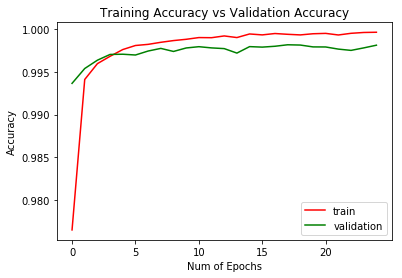
\includegraphics[width=0.6\textwidth]{thesis_template/images/accmnist.png}
    \caption{\small Accuracy of the model during training for 25 epochs on MNIST}
    \label{}
    \end{figure} 
    
\noindent As we can see in the graph the model converged with less number of epochs and has achieved the accuracy of 99.8\% on both train and validation sets. On test set it has achieved accuracy of 99.4\%.
    \begin{figure}[h]
    \centering
    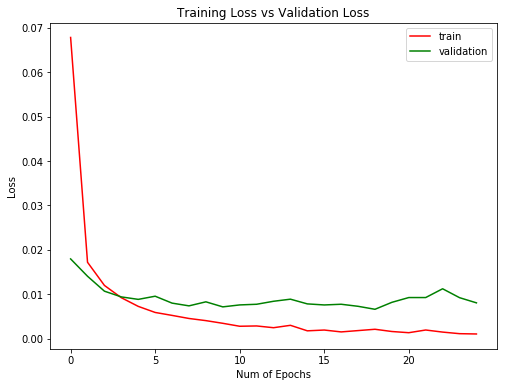
\includegraphics[width=0.5\textwidth]{thesis_template/images/lossmnist.png}
    \caption{\small Variation of loss of the model during training for 25 epochs on MNIST}
    \label{}
    \end{figure}    

\noindent The loss of the model is 0.001\% on train set and 0.006\% on validation set.

\begin{figure}[h]
    \centering
    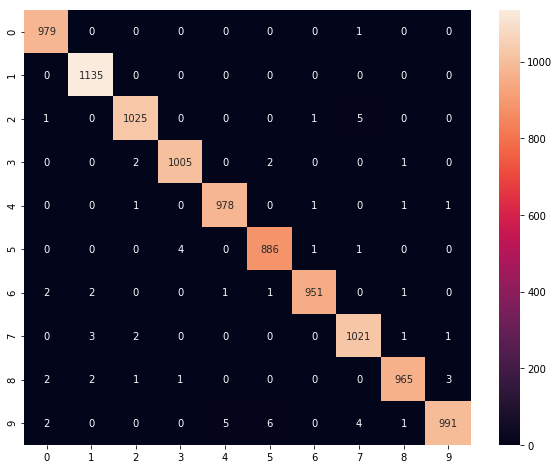
\includegraphics[width=0.6\textwidth]{thesis_template/images/confmatrix.png}
    \caption{\small Confusion-matrix for a model trained for 25 epochs on MNIST}
    \label{}
    \end{figure}

\noindent The image represents the confusion-matrix for the above described model. It represents the number of images that are misunderstood by the model. As we can see rows and columns of classes 0 to 9. Here each row has the actual class and column has predicted class. For example consider row 2 and column 7 has which has a value of 5 it shows how many times model have predicted the images that belong to class 2 as 7.

 One more example for more clear understanding. When we look at the matrix in row 8 and column 3. Here the model have misclassified 1 image of class 8 to class 3. Hence it is clear that even after achieving 99.8\% accuracy there are few wrong predictions. This matrix helps us in calculating other metrics like precision, recall and F1-score. Let us see what are these metrics and why are they used in the next section. The most misclassified class was 9 which is class 10, as we can see in total 18 images are classified wrong.
 
 \begin{table}[h]
\centering
\begin{tabular}{|l|l|l|l|l|}
\hline
          & precision & recall & f1-score & support \\ \hline
0         & 0.99      & 1.00   & 0.99     & 980     \\ \hline
1         & 1.00      & 0.99   & 0.99     & 1135    \\ \hline
2         & 1.00      & 0.99   & 0.99     & 1032    \\ \hline
3         & 0.99      & 1.00   & 0.99     & 1010    \\ \hline
4         & 0.99      & 1.00   & 0.99     & 982     \\ \hline
5         & 1.00      & 0.99   & 0.99     & 892     \\ \hline
6         & 0.99      & 0.99   & 0.99     & 958     \\ \hline
7         & 0.99      & 1.00   & 0.99     & 1028    \\ \hline
8         & 0.99      & 0.99   & 0.99     & 974     \\ \hline
9         & 1.00      & 0.99   & 0.99     & 1009    \\ \hline
avg/total & 0.99      & 0.99   & 0.99     & 10000   \\ \hline
\end{tabular}
\caption{Classification report of model trained for 25 epochs on MNIST}
\end{table}
\noindent The table shows the values of precision, recall and f1-score per class for the test dataset. As we can see the values are between 0.99 and 1.0 which shows that model is very precise. There are very less number False Positives. Apart from these we can see support in the report which indicates the number of actual occurrences of the class in the specified dataset. 
\begin{figure}[h]
    \centering
    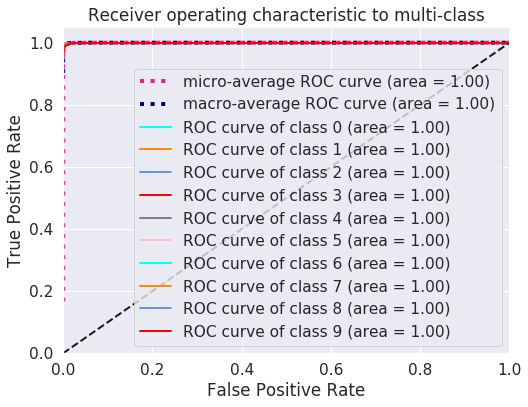
\includegraphics[width=0.8\textwidth]{thesis_template/images/roc.png}
    \caption{\small AUC-ROC graph of the model after 25 epochs}
    \label{}
    \end{figure}
    
\newpage \noindent Since it is a multi-class classifier it looks a bit hard to see all the curves but from the values represented on the right side shows that the value of ROC is always near 1.0 for all the classes which shows that the model is good. This explains that the AUC for all the classes is also 1.0. Since it is a multi-class classifier we also need micro and macro averaged ROC curves.  Micro and macro indicate slightly two different things. A macro average computes ROC independently for each class and then take the average, whereas micro average calculates the aggregate values together and then averages it. This helps us to find out if there is an imbalance in different classes. \\

\noindent Now let us take a look at feature maps for a particular image when passed through this model.



\begin{figure}[h]
    \centering
    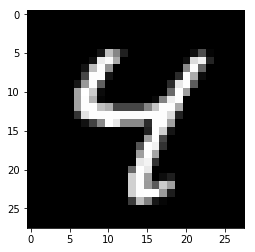
\includegraphics[width=0.4\textwidth]{thesis_template/images/4.png}
    \caption{\small Image 1 selected to visualize}
    \label{}
    \end{figure}


\begin{figure}[h!]
    \centering
    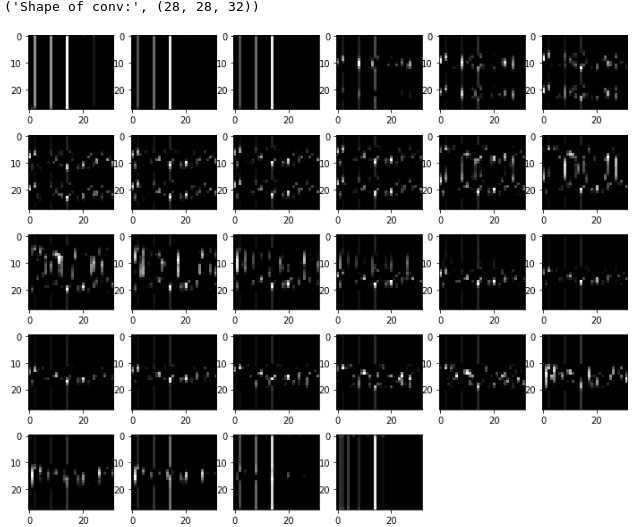
\includegraphics[width=1.0\textwidth]{thesis_template/images/filters.png}
    \caption{\small Filters of first activation layer for image 1}
    \label{}
    \end{figure}


\newpage \noindent  These are the 28 random activations in the first layer, as we can see the visualizations are not clear and it is hard to tell which pattern is recognized by the filters inside that layer. And there are some redundant filters as well for example the first three filters look the same it interprets that they recognize the same patterns. As per previous works the intermediate layers were supposed to recognize low level patterns but here these feature maps does not seem to recognize the patterns of input image. Now let us look at the second layer activations for the same image.


 \begin{figure}[h]
    \centering
    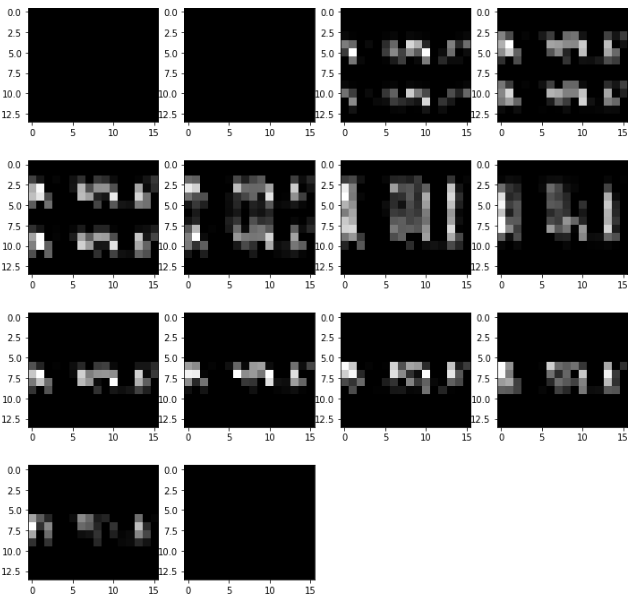
\includegraphics[width=1.0\textwidth]{thesis_template/images/layer2.png}
    \caption{\small Filters of second activation layer for image 1}
    \label{}
    \end{figure}

\newpage \noindent These are 14 random filters taken from the model after second convolution and activation. As per working mechanism of a convnet model the second layer activations depend on first layer so that is the reason why even these filters does not really depict anything. And as we can see there are three \textit{dead filters}. The blank images are considered as dead-filters because we can see that there is no pattern recognized and it looks completely blank. The filters also look very noisy which is a sign that network has not been trained long enough. \\
The third layer visualizations for the image also gave similar activations but just the shape was reduced because of the down sampling of image size. 




It could be the problem of image or the network might be biased for some images so let us look at the activations for another random image from the dataset. 


  \begin{figure}[h]
    \centering
    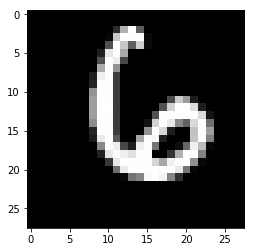
\includegraphics[width=0.5\textwidth]{thesis_template/images/6.png}
    \caption{\small Image 2 selected to visualize}
    \label{}
    \end{figure}
\newpage \noindent This image that belongs to different class and it was chosen randomly from test set. It generated the following visualizations after first activation.

\begin{figure}[h]
    \centering
    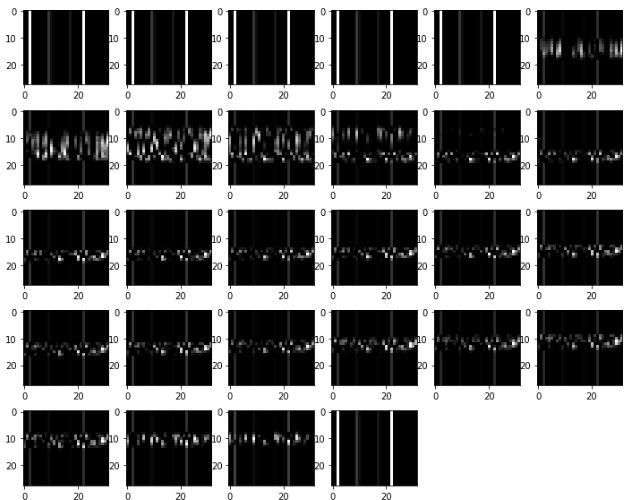
\includegraphics[width=0.8\textwidth]{thesis_template/images/6filers.png}
    \caption{\small First layer activations of image 2 }
    \label{}
    \end{figure}
    
\noindent The activations does not look like the patterns that are present in the input image. And most of the filters look similar it interprets the redundancy in the network. 

 \noindent PS: Even the second layer visualizations for the image looks similar to the first image that is the reason why they are not included here. It has 3 \textit{dead-filters}

\noindent Testing the same method on many different images from the test set showed similar activation filters. Not only this even the train images has shown few dead filters this show that the model has not converged properly and it cannot generalize well.

This indicates that though different performance metrics like accuracy, precision, recall are high there is a need to visualize filters. This is because the model described in the previous section has achieved an accuracy of 99.8\% but ended up with few dead-filters inside the network. In order achieve a model with good filters the model is modified slightly and trained it on more number of \textit{epochs} and less \textit{batch-size}.
\section{Upgraded Model}
In the previous section the model had \textit{Four Convolutional layers} each layer followed by \textit{Relu} and \textit{Max-pooling} layers. Here \textit{Batch-Normalization} layer is added after each Convolution layer and before Relu layer. According to \cite{Sergey} adding BN to the neural network helps us overcome problems with training the network and reduces the dependence of gradients on initial values. To increase the stability of networl BN normalizes the output of previous layer by substracting the batch mean and dividing batch standard deviation. It also makes sure that there is no activation that is either high nor low and thereby even the untrained parameters start to train. This could help us overcome more number of \textit{dead-filters} from the previous model. This model has following parameters.
\begin{itemize}
\item Dataset: MNIST
    \item Activation: Relu
    \item Optimizer: Adam
    \item Batch Normalization
    \item Filter-size: $3 \times 3$, Stride: 1, Padding: Zero
    \item Trained for 100 epochs 
    \item Batch-size: 32
    \item Number of filters remained same as previous model
    \item Dropout: 0.5\%
\end{itemize}

 \noindent Applying these parameters the model has achieved same accuracy of 99.8\%. The graph below represents the variation of accuracy and loss during training.
 \begin{figure}[h!]
    \centering
    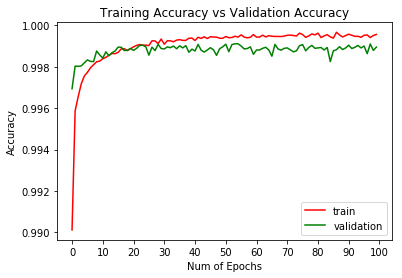
\includegraphics[width=0.8\textwidth]{thesis_template/images/100train.png}
    \caption{\small variation of accuracy during training}
    \label{}
    \end{figure}
\noindent As we can see both on train and validation datasets the accuracy had increased and decreased a bit but achieved maximum accuracy on both datasets.

 \begin{figure}[h!]
    \centering
    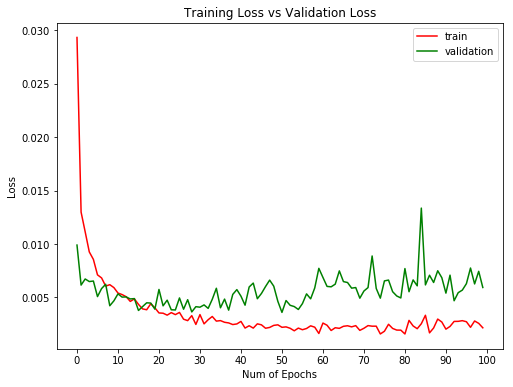
\includegraphics[width=0.8\textwidth]{thesis_template/images/100loss.png}
    \caption{\small variation of loss during training}
    \label{}
    \end{figure}
\newpage\noindent Here the loss on validation has variated more and the model has achieved loss of 0.004\%.

\begin{figure}[h!]
    \centering
    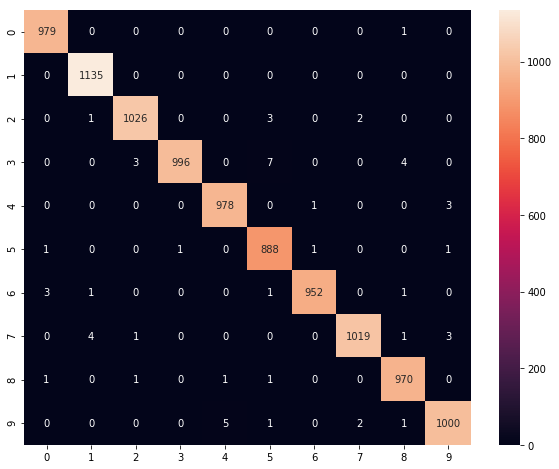
\includegraphics[width=0.85\textwidth]{thesis_template/images/con2.png}
    \caption{\small Confusion-matrix for modified model on test dataset}
    \label{}
    \end{figure}
\newpage\noindent Compared to confusion-matrix of previous model this model has a bit better classification of images. Because there are still images from each class that are misclassified. For example in the previous model and for "class 10" 18 images were predicted wrong, here 9 images were misclassified. This explains that parameters like batch-normalization and increasing epochs does not have much effect on entire performance of the model.
\begin{table}[h!]
\centering
\begin{tabular}{|l|l|l|l|l|}
\hline
          & precision & recall & f1-score & support \\ \hline
0         & 0.99      & 1.00   & 0.99     & 980     \\ \hline
1         & 0.99      & 1.00   & 1.00     & 1135    \\ \hline
2         & 1.00      & 0.99   & 0.99     & 1032    \\ \hline
3         & 0.99      & 1.00   & 0.99     & 1010    \\ \hline
4         & 0.99      & 1.00   & 0.99     & 982     \\ \hline
5         & 1.00      & 0.99   & 0.99     & 892     \\ \hline
6         & 0.99      & 0.99   & 0.99     & 958     \\ \hline
7         & 0.99      & 1.00   & 0.99     & 1028    \\ \hline
8         & 0.99      & 0.99   & 0.99     & 974     \\ \hline
9         & 1.00      & 0.99   & 0.99     & 1009    \\ \hline
avg/total & 0.99      & 0.99   & 0.99     & 10000   \\ \hline
\end{tabular}
\caption{Classification-report for upgraded model trained for 100 epochs on MNIST}
\end{table}
    
 \newpage\noindent The values of precision,recall and f1-score did not change much when compared to the previous model.\\   


\begin{figure}[h]
    \centering
    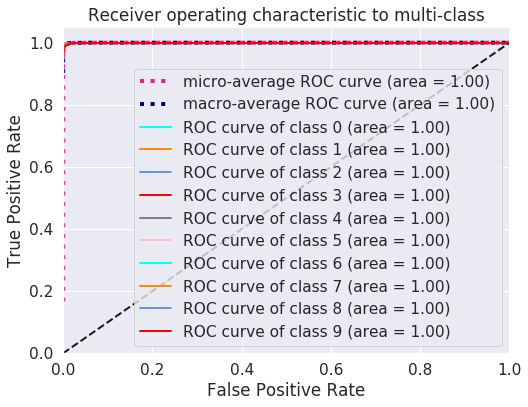
\includegraphics[width=0.6\textwidth]{thesis_template/images/roc.png}
    \caption{\small AUC-ROC curve for upgraded model trained for 100 epochs on MNIST}
    \label{}
    \end{figure}


\noindent Lastly, The AUC-ROC curve for both the models looks same. The AUC(Area Under Curve) for all the classes is 1 which indicates that the model is performing very well. Let us look at the visualizations of the upgraded model. 

\newpage\noindent Following image is selected from the test set

\begin{figure}[h!]
    \centering
    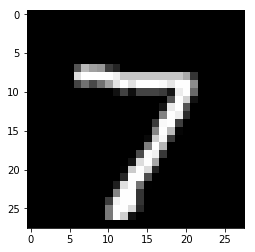
\includegraphics[width=0.3\textwidth]{thesis_template/images/7.png}
    \caption{\small Image 1 for Model 2}
    \label{}
    \end{figure}
 \noindent The image generated the following features in the first activation layer.   
    \begin{figure}[h!]
    \centering
    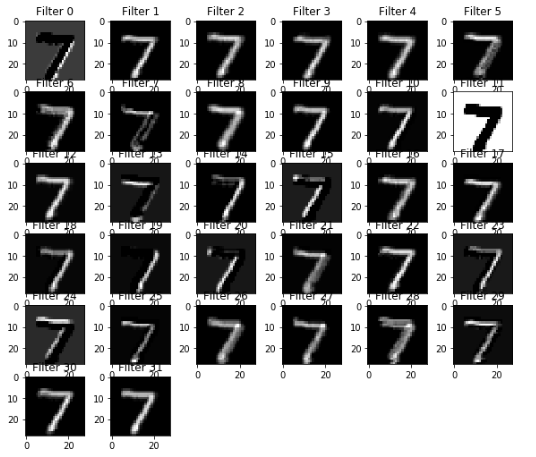
\includegraphics[width=0.9\textwidth]{thesis_template/images/71vis.png}
    \caption{\small First layer visualizations of model 2}
    \label{}
    \end{figure}

\newpage \noindent The first layer looks directly at the raw image pixels. At that stage, the activations are still retaining almost all of the information present in the initial picture. All the 32 filters are trained and there are no dead-filters. The activations are also more clear. Now let us see how the filters change as we go deeper in to the network.

    
\begin{figure}[h]
    \centering
    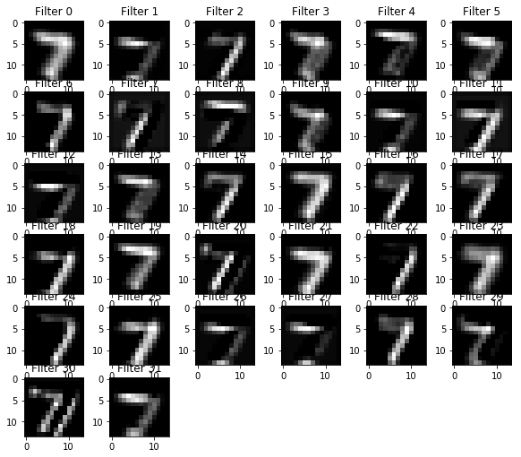
\includegraphics[width=1.0\textwidth]{thesis_template/images/72vis.png}
    \caption{\small Second layer visualizations of model 2}
    \label{}
    \end{figure}

\newpage \noindent The image represents the filters after second activation. All the filters are trained which is indication of no dead-filters. The white part inside each filter represents the pattern of the input image. We can notice that as we go deeper in to the model the filters look less like original image and has more abstract representation. Here all the filters are looking for almost similar type of patterns from input image. Let us see how there patterns are shared between 64 filters in the next convolution layer.


\begin{figure}[h]
    \centering
    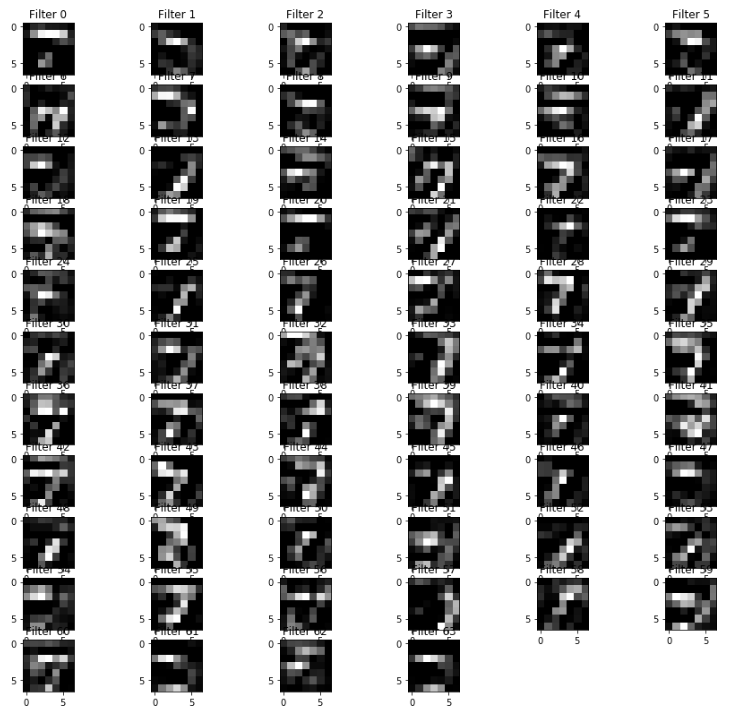
\includegraphics[width=0.95\textwidth]{thesis_template/images/73.png}
    \caption{\small Third layer visualizations of model 2}
    \label{}
    \end{figure}
 
 \newpage \noindent As we can see the filters in this layer are looking for variety of patterns from the input image. Now the difference can be seen as the presence of original image is much harder to see in these filters. It is a good indication that all the patterns are activated in different filters. For most of the features it is easy to say what part of image activated them. In order to show that the network is not biased one more image and its activations are shown here.
\begin{figure}[h]
    \centering
    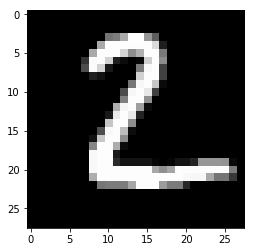
\includegraphics[width=0.5\textwidth]{thesis_template/images/2.png}
    \caption{\small Image 2}
    \label{}
    \end{figure}
\newpage The first three layer filters are shown below.
\begin{figure}[h!]
    \centering
    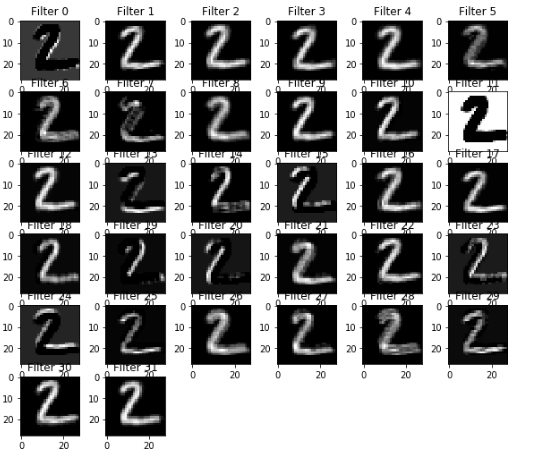
\includegraphics[width=0.95\textwidth]{thesis_template/images/21.png}
    \caption{\small first layer visualizations of model 2 for image 2}
    \label{}
    \end{figure}
    
\begin{figure}[h]
    \centering
    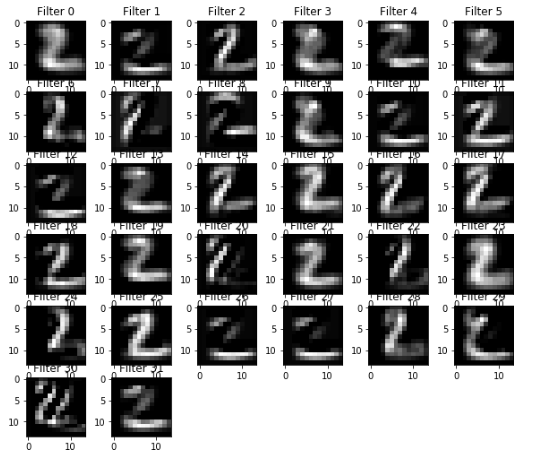
\includegraphics[width=1.0\textwidth]{thesis_template/images/22.png}
    \caption{\small Second layer visualizations of model 2 for image 2}
    \label{}
    \end{figure}
\newpage \noindent Both the layers does not contain any dead-filters. It is so clear that since the network has given 2 as input image most of the filters are activated in such a way that they produce high value for 2. Since the network is responsible to classify it as 2. It generates high outputs for 2s by having large weights aligned to pixels which tend to usually be high in images of 2s. Simultaneously, it can obtain relatively low outputs for non-2s by having small weights aligned to pixels which tend to be high in images of non-2s and low in images of 2s. One last thing is visualizing the third layer in the network.



\begin{figure}[h]
    \centering
    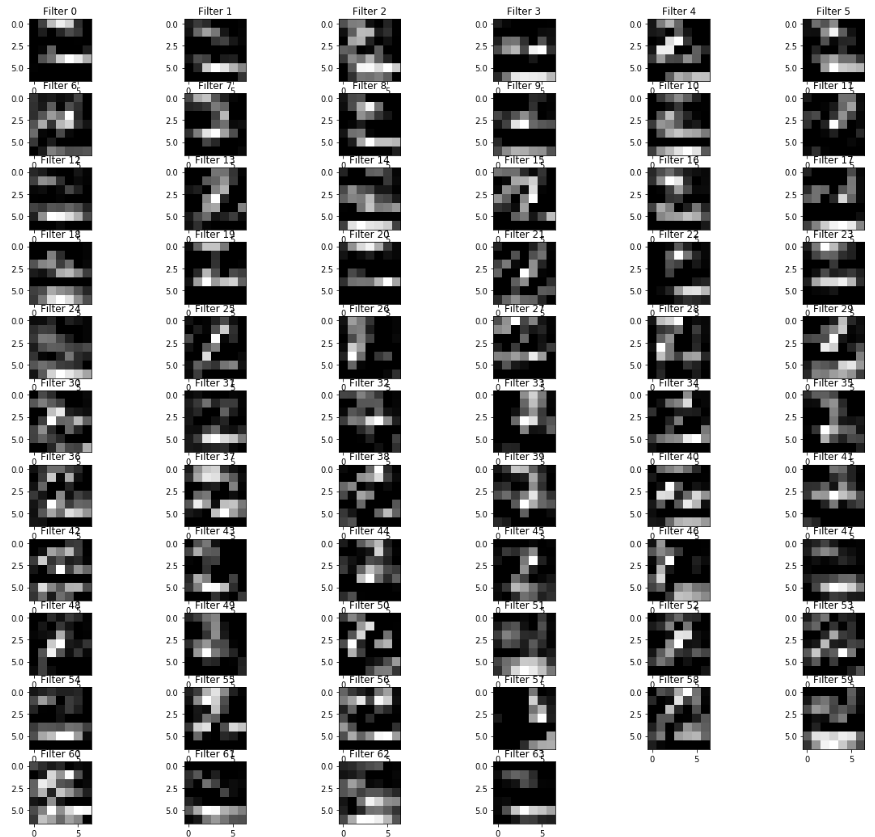
\includegraphics[width=0.9\textwidth]{thesis_template/images/23.png}
    \caption{\small Third layer visualizations of model 2 for image 2}
    \label{}
    \end{figure}
    
\newpage \noindent Some filters look like blurry 2. And the white part inside each filter represents the pixels of the input image that activate them. We can interpret these neurons as forming templates of output. The visualizations indicate that the network has converged. Till now we have seen the visualizations of network trained only on MNIST dataset which is very easy. Now let us look at the filters of the same network which is trained on CIFAR-10 dataset which has images of real world.

\newpage \section{Upgraded Model on CIFAR-10 dataset}
CIFAR-10 consists of 60000 labeled images which are of size $32 \times 32$ and have 3 channels. Here 50000 images belong to train dataset and 10000 belong to test dataset. And these images belong to 10 different classes which are airplanes, automobiles, birds, cats, deer, dogs, frogs, horses, ships, and trucks. The model is same with same parameters which are shown in upgraded model with batch-normalization layer. The model was trained for 100 epochs with batch-size of 32. The model has achieved the accuracy of 88\% on training dataset and loss of 0.3\%. On test dataset the accuracy achieved was 82\%.


\begin{figure}[h]
    \centering
    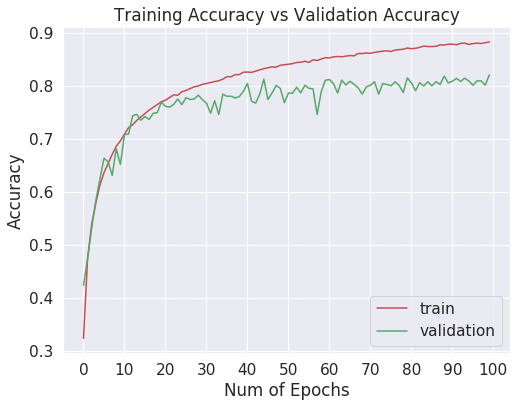
\includegraphics[width=0.52\textwidth]{thesis_template/images/cifacc.png}
    \caption{\small Variation of accuracy during training on CIFAR-10 for 100 epochs}
    \label{}
    \end{figure}

\begin{figure}[h]
    \centering
    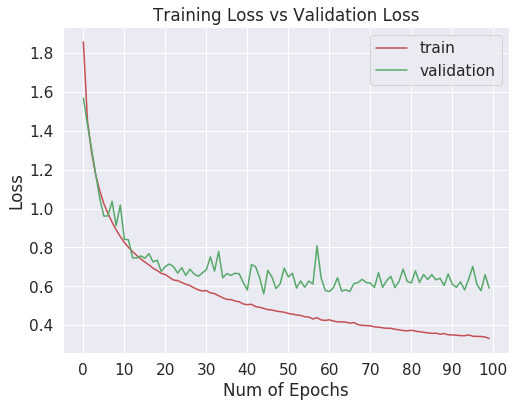
\includegraphics[width=0.52\textwidth]{thesis_template/images/cifloss.png}
    \caption{\small Variation of loss during training on CIFAR-10 for 100 epochs}
    \label{}
    \end{figure}
    
\begin{figure}[h]
    \centering
    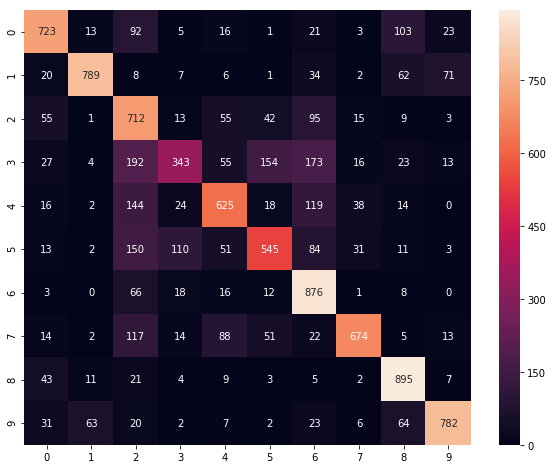
\includegraphics[width=0.7\textwidth]{thesis_template/images/cmcif.png}
    \caption{\small Confusion-matrix for CIFAR-10}
    \label{}
    \end{figure}
\newpage \noindent Here we can see that so many images are predicted wrong. Especially images that belong to class 3 seems to have more False Positives. The same model was unable to infer properly on other dataset. The precision, recall and f1-scores for the model are given below in Table 4.2. The values indicate that the model just has average performance.

\begin{table}[]
\centering
\begin{tabular}{|l|l|l|l|l|}
\hline
          & precision & recall & f1-score & support \\ \hline
0         & 0.77      & 0.72   & 0.74     & 1000     \\ \hline
1         & 0.89      & 0.79   & 0.84     & 1000    \\ \hline
2         & 0.47      & 0.71   & 0.56     & 1000    \\ \hline
3         & 0.64      & 0.35   & 0.45     & 1000    \\ \hline
4         & 0.67      & 0.62   & 0.65     & 1000    \\ \hline
5         & 0.66      & 0.55   & 0.60     & 1000     \\ \hline
6         & 0.60      & 0.88   & 0.71     & 1000     \\ \hline
7         & 0.86      & 0.67   & 0.75     & 1000   \\ \hline
8         & 0.75      & 0.90   & 0.82     & 1000     \\ \hline
9         & 0.85      & 0.78   & 0.82     & 1000    \\ \hline
avg/total & 0.72      & 0.70   & 0.69     & 10000   \\ \hline
\end{tabular}
\caption{Classification-report of upgraded model on CIFAR-10 after training for          100 epochs}
\end{table}

\newpage\begin{figure}[h]
    \centering
    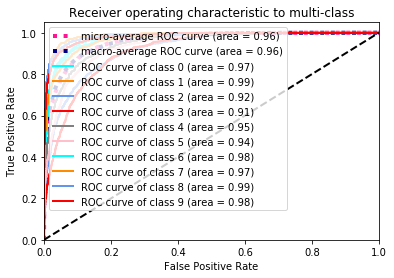
\includegraphics[width=0.68\textwidth]{thesis_template/images/cifroc.png}
    \caption{\small AUC $-$ ROC curve of CIFAR-10 after training for 100 epochs}
    \label{}
    \end{figure}

 \noindent Surprisingly the Area under curve indicates that the model has performed fine on the dataset. Now let us look at the images from the test dataset and the reaction of weights for that image. First image is horse  


\begin{figure}[h]
    \centering
    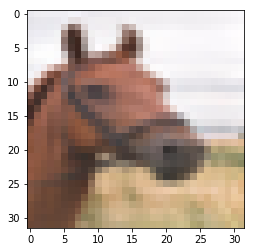
\includegraphics[width=0.45\textwidth]{thesis_template/images/horse.png}
    \caption{\small Horse image from CIFAR-10 }
    \label{}
    \end{figure}
    
\begin{figure}[h]
    \centering
    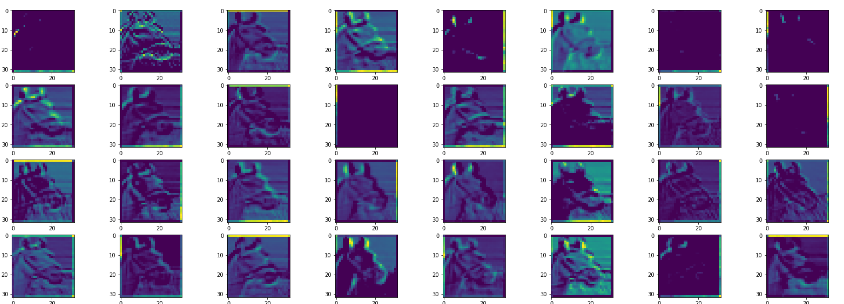
\includegraphics[width=1.0\textwidth]{thesis_template/images/horsefil1.png}
    \caption{\small 32 Filters of layer1}
    \label{}
    \end{figure}

\newpage \noindent All the features represent the input image. As we can see all the filters are activated and more patterns from the input image are seen. Next is second layer visualizations for this image.

\begin{figure}[h]
    \centering
    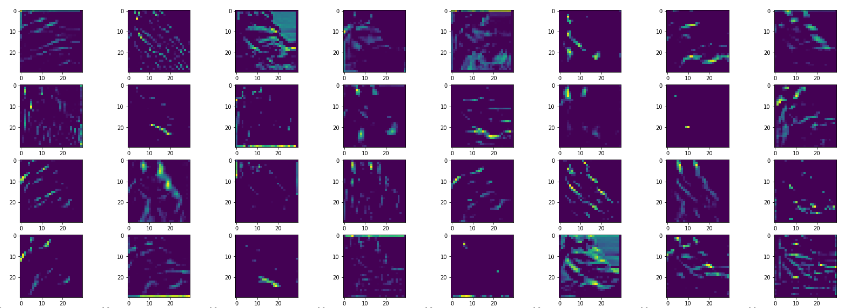
\includegraphics[width=1.1\textwidth]{thesis_template/images/horsefil2.png}
    \caption{\small 32 Filters of layer 2}
    \label{}
    \end{figure}
\newpage \noindent The figure represents the feature maps of layer 2. We can see that the patterns from the input image are less visible but still we can say which patterns activated particular filter. There are no dead-filters in both the layers. Next we will see how third layer visualizations look like.

\begin{figure}[h]
    \centering
    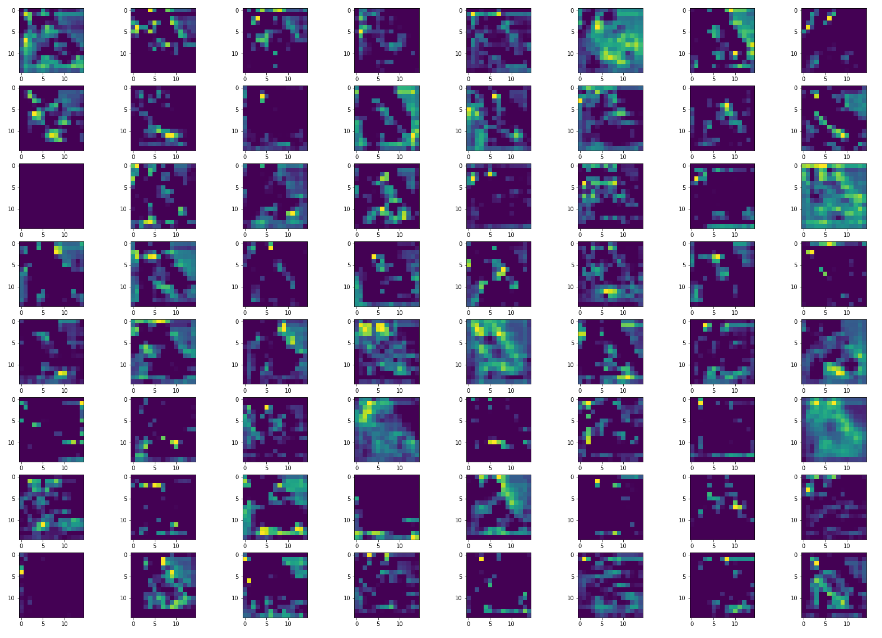
\includegraphics[width=1.0\textwidth]{thesis_template/images/horsefil3.png}
    \caption{\small 64 Filters of layer 3}
    \label{}
    \end{figure}
\newpage \noindent The figure represents all the 64 features from the third layer. It is hard to say which pattern activated the particular filter. The deeper layers encode higher-level features like nose,ears etc that is the reason why these feature maps contain less information about the input image. One more image from the cifar-10 is represented below.


\begin{figure}[h]
    \centering
    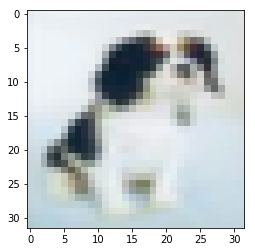
\includegraphics[width=0.45\textwidth]{thesis_template/images/dog1.png}
    \caption{\small Dog image from cifar-10}
    \label{}
    \end{figure}

\newpage\noindent The first layer activations for this image are\\
\begin{figure}[h]
    \centering
    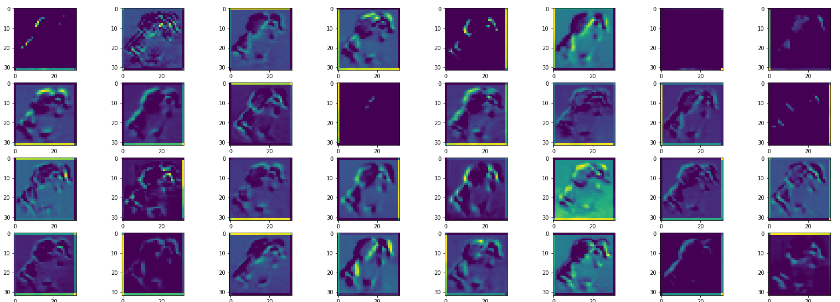
\includegraphics[width=1.1\textwidth]{thesis_template/images/dog1fil1.png}
    \caption{\small 32 Filters of layer 1 for image 2}
    \label{}
    \end{figure}\\
\noindent For both the images taken from cifar-10 dataset in the layer 3 , 17th filter does not activate at all which indicates the dead-filter. But here there is only one dead-filter so this can ignored. The filters of second and third layer for the dog image are shown in the next page.   

\begin{figure}[h]
    \centering
    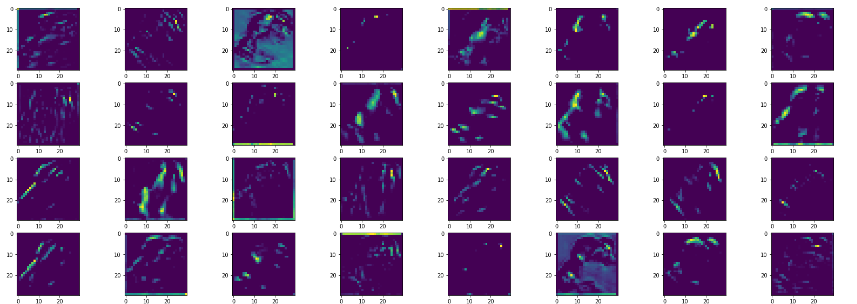
\includegraphics[width=1.0\textwidth]{thesis_template/images/dog1fil2.png}
    \caption{\small 32 Filters of layer 2 for image 2}
    \label{}
    \end{figure}


\begin{figure}[h]
    \centering
    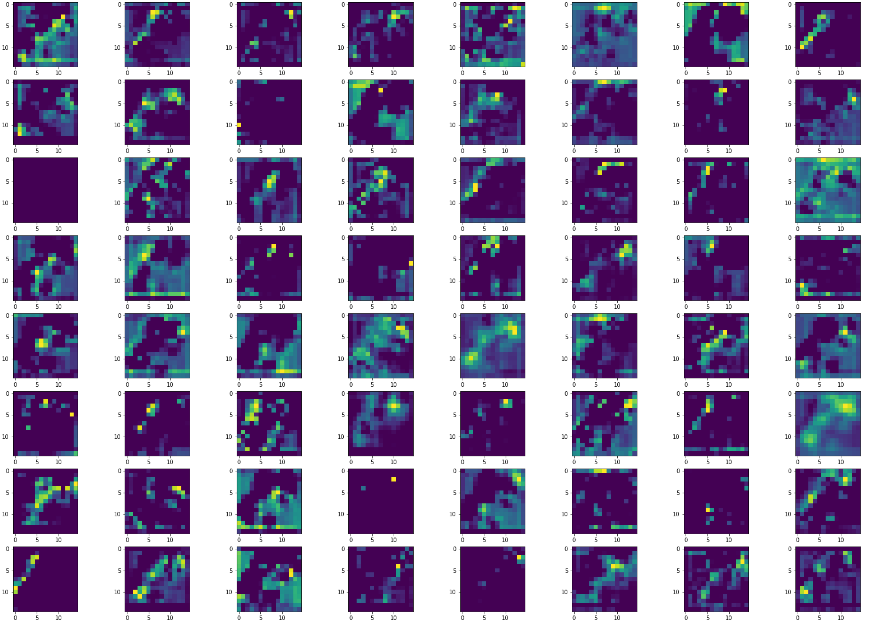
\includegraphics[width=1.0\textwidth]{thesis_template/images/dog1fil3.png}
    \caption{\small 64 Filters of layer 3 for image 2}
    \label{}
    \end{figure}

\chapter{Discussion}\label{chap:discussion}

According to the experience gained from the results we can see that there are few dead-filters in the model which is not trained long enough. In order to evaluate those visualizations I have built a dataset with three labeled classes which are redundant filters, dead-filters and normal filters. But since the dead-filters were only three to four it was not feasible to do image classification. So they are just represented in the form of visualizations. 
\subsubsection{Training time and device used}

The experiments were conducted on CPU with Windows OS and Anaconda environment. The python version used was 3.5.
\begin{itemize}
    \item To train the first model which just had Convolution, max-pooling and Relu layers with the help of Adam optimizer which had learning rate of 0.001 it took 5 hours. It was trained for 25 epochs with batch-size of 200 and MNIST dataset.
    \item To train the upgraded model which just had additional Batch-Normalization layer and dropout layer with 0.5. It was trained for 100 iterations with a batch-size of 32 it took around 12 hours and for same MNIST dataset. It has achieved accuracy of 99.8\%.
    \item But when same model was trained on CIFAR-10 dataset with same number of iterations and batch-size it took around 15 hours and achieved accuracy of 88\% which is less when compared to the previous one.
\end{itemize}

\noindent In order to visualize everything the coding is done using Jupyter Notebook.

\newpage \noindent The following are the observations from the experiments.
\begin{itemize}
    \item Parameters like number of epochs does have an effect on learning patterns of the weights. This is evident when we compare figure 4.2 and figure 4.11.
    \item Addition of Batch-Normalization reduces the dead-filters and redundant filters inside the network.
    \item When we use mini batch-size the weights are trained more effectively and reduces dead-filters. 
    \item The filter-size did not show any effect on the feature maps. Because when the filter size was increased to 5 it showed the similar activations. 
    \item It is clearly evident that the deeper we go in to the network patterns recognized by the weights look more abstract and they contain less information about the input image. It was also stated in previous works.
\end{itemize}



\noindent The filters of upgraded model trained on MNIST dataset represent more obvious patterns from the input image. But for a dataset like CIFAR-10 the filters are not so clear though there are no dead-filters spotted the visualizations are very noisy. Adding more regularizations like L2 to the network might help them overcome these noisy patterns and get more smooth filters. This concludes one more point which is each dataset needs different type of regularization parameters. And one last thing is evaluating the model on higher resolution images might give out filter visualizations which are more clear. Then the feature maps would be more apparent. 


\chapter{Conclusion}\label{chap:conclusion}
 In this thesis we addressed the main pitfall of Convnets. And how it can be solved by visualizing them.  Our contribution does not include proposing a new method to visualize the hidden layers in the network as there are already so many existing methods. It only shows which is the easy method to see each and every filter in the intermediate layers which is explained in Chapter 3. Most importantly we have shown that the parameters like number of epochs, batch-size does have an effect on pattern recognition part of the network. It is evident when we look the visualizations of two different models which are shown in chapter 4. In order to look for dead or redundant filters we need to visualize all the filters in the layers that is the reason why we have chosen to plot each individual filter as an image. 
 Addition of Batch-Normalization and Dropout layer yielded more better and clearer visualizations of the filters.  
 
 \section{Future Work}
The main intention of this thesis is to provide a basic knowledge about pattern recognition nature of filters. Many different experiments are left for future due to lack of time. The following are the ideas that can be tested in future:
\begin{itemize}
    \item Extend this experiments on high resolution image datasets. Due to hardware and time constraints this work included only low resolution image datasets.
    \item Try adding L1 and L2 regularization techniques and check if they provide more smooth filters.  
    \item Build a new model with different stride values and analyze their effect.
   
\end{itemize}



\noindent Here we were able to do only qualitative evaluation of these visualizations based on the previous research papers. This can be extended by introducing more robust and general methods for quantitative evaluation of these visualizations. 

The experimental results of this work are not satisfactory and further study is definitely required in order to get deeper insights in to the parameters that contribute to the pattern recognition nature of these filters. The contribution of this thesis alone is not enough to build real world models. The work can also be extended by testing many different combinations of parameters like learning rates, activation functions, optimizers and find out the best one which yields good visualizations. I believe that if we use better and faster processing units like GPUs and TPUs there is much scope for further experimentation.



% -- Appendix (optional)
\begin{appendices}
    % !TeX spellcheck = en_US
% !TeX encoding = UTF-8

\end{appendices}
\newpage


%%%%%%%%%%%%%%%%%%%%%%%%%%%%%%%%%%%%%%%%%%%%%%%%%%%%%%%%%%%%%%%%%%%%%%%%%%%%%%%%%%%%%%%%%
\backmatter

% -- Bibliography
\printbibliography

% -- Eidesstattliche Erklärung (= Affadavit)


\end{document}